% This is the Reed College LaTeX thesis template. Most of the work
% for the document class was done by Sam Noble (SN), as well as this
% template. Later comments etc. by Ben Salzberg (BTS). Additional
% restructuring and APA support by Jess Youngberg (JY).
% Your comments and suggestions are more than welcome; please email
% them to cus@reed.edu
%
% See https://www.reed.edu/cis/help/LaTeX/index.html for help. There are a
% great bunch of help pages there, with notes on
% getting started, bibtex, etc. Go there and read it if you're not
% already familiar with LaTeX.
%
% Any line that starts with a percent symbol is a comment.
% They won't show up in the document, and are useful for notes
% to yourself and explaining commands.
% Commenting also removes a line from the document;
% very handy for troubleshooting problems. -BTS

% As far as I know, this follows the requirements laid out in
% the 2002-2003 Senior Handbook. Ask a librarian to check the
% document before binding. -SN

%%
%% Preamble
%%
% \documentclass{<something>} must begin each LaTeX document
\documentclass[12pt,twoside]{templates/facsothesis}
% Packages are extensions to the basic LaTeX functions. Whatever you
% want to typeset, there is probably a package out there for it.
% Chemistry (chemtex), screenplays, you name it.
% Check out CTAN to see: https://www.ctan.org/
%%
\ifxetex
  \usepackage{polyglossia}
  \setmainlanguage{spanish}
  % Tabla en lugar de cuadro
  \gappto\captionsspanish{\renewcommand{\tablename}{Tabla}
          \renewcommand{\listtablename}{Índice de tablas}}
\else
  \usepackage[spanish,es-tabla]{babel}
\fi
%\usepackage[spanish]{babel}
\usepackage{graphicx,latexsym}
\usepackage{amsmath}
\usepackage{amssymb,amsthm}
\usepackage{longtable,booktabs,setspace}
\usepackage{chemarr} %% Useful for one reaction arrow, useless if you're not a chem major
\usepackage[hyphens]{url}
% Added by CII
%\usepackage{hyperref}
\usepackage[colorlinks = true,
            linkcolor = blue,
            urlcolor  = blue,
            citecolor = blue,
            anchorcolor = blue]{hyperref}
\usepackage{lmodern}
\usepackage{float}
\floatplacement{figure}{H}
% End of CII addition
\usepackage{rotating}
\usepackage{placeins} % para fijar la posición de las tablas con \FloatBarrier


\usepackage[]{natbib}


% Next line commented out by CII
%\usepackage{biblatex}
%\usepackage{natbib}
% Comment out the natbib line above and uncomment the following two lines to use the new
% biblatex-chicago style, for Chicago A. Also make some changes at the end where the
% bibliography is included.
%\usepackage{biblatex-chicago}
%\bibliography{thesis}


% Added by CII (Thanks, Hadley!)
% Use ref for internal links
\renewcommand{\hyperref}[2][???]{\autoref{#1}}
\def\chapterautorefname{Chapter}
\def\sectionautorefname{Section}
\def\subsectionautorefname{Subsection}
% End of CII addition

% Added by CII
\usepackage{caption}
\captionsetup{width=5in}
% End of CII addition

% \usepackage{times} % other fonts are available like times, bookman, charter, palatino

% Syntax highlighting #22

% To pass between YAML and LaTeX the dollar signs are added by CII
\title{{ Desigualdad, política y lenguaje}: El rol del manejo del lenguaje en la transmisión intergeneracional de las habilidades políticas en jóvenes chilenos}
\author{Francisco Javier Meneses Rivas}
% The month and year that you submit your FINAL draft TO THE LIBRARY (May or December)
\date{Santiago de Chile, año 2022}
\division{}
\advisor{Profesor guía
Juan Carlos Castillo}
\institution{Universidad de Chile}
\degree{Tesis para optar al grado de Magister en Ciencias Sociales}
%If you have two advisors for some reason, you can use the following
% Uncommented out by CII
% End of CII addition

%%% Remember to use the correct department!
\department{}
% if you're writing a thesis in an interdisciplinary major,
% uncomment the line below and change the text as appropriate.
% check the Senior Handbook if unsure.
%\thedivisionof{The Established Interdisciplinary Committee for}
% if you want the approval page to say "Approved for the Committee",
% uncomment the next line
%\approvedforthe{Committee}

% Added by CII
%%% Copied from knitr
%% maxwidth is the original width if it's less than linewidth
%% otherwise use linewidth (to make sure the graphics do not exceed the margin)
\makeatletter
\def\maxwidth{ %
  \ifdim\Gin@nat@width>\linewidth
    \linewidth
  \else
    \Gin@nat@width
  \fi
}
\makeatother

%Added by @MyKo101, code provided by @GerbrichFerdinands

\setlength\parindent{0pt}


% Added by CII

\providecommand{\tightlist}{%
  \setlength{\itemsep}{0pt}\setlength{\parskip}{0pt}}

\Acknowledgements{

}

\Dedication{

}

\Preface{

}

\Abstract{

}

% End of CII addition
%%
%% End Preamble
%%
%
\let\chaptername\relax
\begin{document}
\bibliographystyle{apalike}
% Everything below added by CII
  \maketitle

\frontmatter % this stuff will be roman-numbered
\pagestyle{empty} % this removes page numbers from the frontmatter



%  \hypersetup{linkcolor=black}
  \setcounter{tocdepth}{1}
  \setlength{\parskip}{0pt}
  \tableofcontents

\setlength\parskip{1em plus 0.1em minus 0.2em}

  \listoftables

  \listoffigures



\mainmatter % here the regular arabic numbering starts
\pagestyle{fancyplain} % turns page numbering back on

\hypertarget{resumen}{%
\chapter*{Resumen}\label{resumen}}
\addcontentsline{toc}{chapter}{Resumen}

Actualmente las democracias se encuentran frente a una crisis de legitimidad que se relaciona, entre otras cosas, con la falta de representación de distintos grupos, como los sectores populares y los jóvenes. Al respecto, las investigaciones han señalado que no solo existen diferencias actitudinales hacia la política según grupo social, sino que también existen brechas en las habilidades políticas que se relacionan con la participación desigual. La asociación internacional para la evaluación del logro educativo (IEA) ha desarrollado el Estudio Internacional de Educación Cívica y Formación Ciudadana (ICCS) que se enfoca en estudiar las Habilidades y Conocimientos necesarios para la vida ciudadana en jóvenes estudiantes. El conocimiento cívico de la ICCS ha generado interés en distintos investigadores puesto que se asocia positivamente con un conjunto de actitudes democráticas como la participación y la tolerancia. Se ha demostrado que existe una relación entre nivel socioeconómico y conocimiento Cívico. Al explicar esta desigualdad algunos autores han señalado que en familias de alto capital cultural se genera un ambiente más ciudadano y académico, que implica una socialización en valores políticos y habilidades cognitivas. Para profundizar esta línea de investigación, se propone que parte de lo que explica la relación entre desigualdad social y conocimiento cívico es el manejo del lenguaje, esto basado en una visión sociológica del lenguaje como elemento cohesionador, crítico y transmisible. Para evaluar esta hipótesis se trabajaron conjuntamente los datos de la ICCS y el SIMCE (N = 3140). A partir de los análisis de mediación multinivel, se concluye que la transmisión intergeneracional de la desigualdad habilidades políticas se explica más por habilidades en el lenguaje que por la transmisión de intereses político. Además, se evidencia el potencial del lenguaje para disminuir la desigualdad de habilidades políticas, lo cual debe considerarse para la implementación del ramo de formación ciudadana.

Palabras clave: Conocimiento Cívico, Desigualdad política, Comprensión lectora, Interés político

\hypertarget{agradecimientos}{%
\chapter*{Agradecimientos}\label{agradecimientos}}
\addcontentsline{toc}{chapter}{Agradecimientos}

Deseo profundamente poder agradecer en estas páginas a más de las personas de las que caben en ellas. Por lo pronto, es menester agradecer a mis padres que con su esfuerzo pudieron educarme y darme con ello mejores posibilidades de vida.
Agradecer directamente a mi pareja Anais Herrera junto con quien desperté el interés por la sociología y junto a quien he tenido las reflexiones que han dado vida a esta tesis.

También quiero agradecer muy sinceramente al profesor Juan Carlos Castillo quien me ha ayudado a profesionalizarme en estos últimos años y quien me presentó el marco de investigación al que intenta aportar esta tesis. En la misma línea quisiera agradecer a Felipe Ruiz que fue el primero en dedicarse a enseñarme el uso del Software R el cual ha sido mi herramienta fundamental de trabajo. Finalmente deseo agradecer a Julio Iturra como mi primer colega de trabajo de quién aprendido muchas cosas prácticas que no se incorporaron en mi formación universitaria.

Fuera de lo personal deseo agradecer a todas las personas y científicos que han contribuido a la construcción colectiva del conocimiento. Agradecer especialmente a quienes en consonancia con la ciencia abierta han compartido sus conocimientos ayudándome progresar. Entre ellos agradezco especialmente a Yihui Xie quien ha democratizado múltiples herramientas digitales, haciéndolas más fáciles de usar sin la necesidad de ser un erudito de la programación.

\hypertarget{introducciuxf3n}{%
\chapter{Introducción}\label{introducciuxf3n}}

Construir sociedades más democráticas es un objetivo internacional consagrado por la Organización de las Naciones Unidas tanto en la Declaración Universal de los Derechos Humanos como en el Pacto internacional de los Derechos Civiles y Políticos. Basándose en estos tratados internacionales, para que una sociedad sea efectivamente democrática son requisitos fundamentales una amplia participación de la ciudadanía y que la participación sea representativa, es decir, que no tenga sesgos socioeconómicos, raciales, de género, o de cualquier otra razón. Actualmente podemos decir que múltiples democracias poseen conflictos respecto a estas dos condiciones. En primer lugar, existe una tendencia a la disminución en la participación politica \citep{tezanos-pinto_Participacion_2015, herrmann_Disminucion_2016, diaz_Dimensiones_2017, janmaat_Civic_2013, contreras_DIFERENCIAS_2013, galston_Civic_2007}. En segundo lugar, la participación politica es desigual, perjudicando la representación de la voz politica de sectores más pobres, de grupos racializados, de las mujeres y de los más jóvenes \citep{verba_Would_2003, lijphart_Unequal_1997, desposato_Gender_2009, coffe_Explaining_2020, hutchings_CENTRALITY_2004}. Más aun, estas desigualdades políticas se transmiten de manera intergeneracional \citep{brady_Political_2015}. En el caso Chileno, tanto el Centro de Estudio de Conflicto y Cohesión Social (COES) como el Programa de las Naciones Unidas para el Desarrollo (PNUD) han señalado que existe una gran desigualdad en la participación política, la cual sobrerrepresenta los grupos acomodados del país favoreciendo la reproducción de la desigualdad \citep{joignant_Desigualdades_2017, palet_Desiguales_2017}.

Con el objetivo de fomentar valores democráticos en los ciudadanos y afrontar los desafíos de las democracias, cada vez más países, entre ellos chile, han incorporado en sus planes de estudio un mayor espacio para temáticas ciudadanas \citep{keer_ciudadania_2015}. La escuela es un lugar estratégico para fomentar valores, principios y conductas democráticas, pues en ella se realiza un proceso de socialización donde los estudiantes incorporan normas sociales necesarias para la vida en su comunidad \citep{durkheim_Educacion_2010}. En torno a la socialización ciudadana de los jóvenes en las escuelas existen más de cuarenta años acumulados de investigaciones desde las ciencias sociales \citep{torney_Crossnational_1979}. Estas investigaciones han evidenciado reiteradamente que los estudiantes de distintos grupos socioeconómicos poseen distintas actitudes e intenciones de participación, lo cual es un obstáculo para la realización de la democracia \citep{castillo_Social_2014, miranda_Political_2018, ferrans_Civic_2017, trevino_Influence_2017}.

Además de estudiar las actitudes y conductas políticas de los estudiantes, desde 1990, existe un esfuerzo por medir y estudiar las capacidades cognitivas de los jóvenes para su vida ciudadana \citep{torney-purta_estudio_2015}. Este esfuerzo derivó en la prueba de conocimiento Cívico y Ciudadano la cual fue aplicada en tres encuestas internacionales de formación cívica. Según los creadores de la escala, esta busca medir tanto el conocimiento que poseen los estudiantes de sus sistemas políticos, como las habilidades cognitivas que poseen para reflexionar sobre situaciones concretas a partir de principios democráticos y su conocimiento político \citep{schulz_Initial_2010}. Existe contundente evidencia para señalar que un mayor conocimiento cívico se relaciona con mejores actitudes democráticas como la participación y la tolerancia \citep{schulz_Initial_2010, galston_Civic_2007, miranda_Political_2018}. Una de las conclusiones más relevante de estos estudios es que existe una transmisión intergeneracional de la desigualdad politica, es decir, estudiantes hijos de padres con mejor situación económica, posen mejores conocimientos y habilidades para desenvolverse en la vida politica \citep{schulz_Initial_2010, miranda_Desigualdad_2015}. Respecto a esta desigualdad, si bien se ha señalado que está estrechamente relacionada con aspectos de desigualdad cultural (p.~ej. Educación de los padres y cantidad de libros en el hogar) y transmisión de actitudes, se ha dado poca relevancia a la transmisión de habilidades que ayudan a reproducir la desigualdad en la política \citep{brady_Political_2015}. En torno a las habilidades, la organización de Estados Americanos (OEA) señala que la carencia en alfabetización puede ser un obstáculo para la educación cívica en Chile \citep{torney-purta_estudio_2015}. Esta advertencia de la OEA, y algunas investigaciones que demuestran la dificultad de los estudiantes al leer la prueba por el lenguaje relativamente abstracto y complejo \citep{zhang_Understanding_2015, arensmeier_Swedish_2015}, sugieren que el manejo del lenguaje posee un rol relevante para comprender las abstractas temáticas ciudadanas jugando un rol en la reproducción de la desigualdad política.

En consideración de lo señalado, la pregunta de esta investigación es:

\begin{quote}
¿Cuál es el rol que juega el manejo del lenguaje en la transmisión intergeneracional de la desigualdad politica?
\end{quote}

Esta investigación busca evidenciar la importancia del manejo del lenguaje para explicar las desigualdades en habilidades políticas, frente a otras explicaciones alternativas basadas en la trasmisión de valores democrticos. Al explicar la reproducción intergeneracional de los conocimientos y habilidades políticas, las investigaciones recurren a dos líneas teóricas de la socialización: \emph{la actitudinal}, centrada en la transmisión de valores e intereses, y \emph{la cognitiva}, centrada en la transmisión de habilidades \citep{miranda_Political_2018}. La propuesta de esta investigación plantea que la desigualdad de las habilidades cívico-ciudadanas se explica en una buena medida por desigualdades en habilidades, y más específicamente, por el manejo del lenguaje.

Esta propuesta no solo se sustenta en el efecto de la cultura académica de los padres en las habilidades políticas, sino también en que la comprensión lectora requiere de las mismas destrezas cognitivas que el conocimiento cívico (Ej. Comprender, interpretar, analizar, evaluar, entre otras). Por ejemplo, para que un joven logre identificar una acción como antidemocrática, como alguien insultando a un inmigrante por su origen, no solo debe ser capaz de comprender que una persona le grita a otra, sino que debe \emph{interpretar} cual es el sentido de esa acción y ser capaz de \emph{evaluar la relación} entre dicho sentido y los principios democráticos, habilidades semejantes a las necesarias para la comprensión lectora. De este modo, para poseer un buen conocimiento cívico no solo es necesario poseer valores ciudadanos, sino habilidades reflexivas del lenguaje.

El considerar que la comprensión de la vida cívica puede estar asociada a la comprensión del lenguaje no solo es relevante dentro del campo de la educación, sino también en el campo de la acción política y la democracia. Si un joven es capas de comprender mediante el lenguaje distintos ideales democráticos es más probable que actúe y opine en concordancia con ellos. Más aun, el comprender distintos ideales puede abrir las posibilidades de acción del sujeto ya que, la si la realidad es social y construida mediante el lenguaje, poseer un mayor manejo del lenguaje implica una mayor capacidad reflexiva sobre la realidad, una mayor capacidad critica y, por ende, una mayor capacidad de agencia. El lenguaje no solo nos permite enunciar el mundo, sino que tambien nos ayuda a analizarlo, criticarlo y así actuar reflexivamente sobre él.

En suma, se propone que el manejo del lenguaje posee una mejor capacidad mediadora que otras variables usualmente consideradas relevantes para explicar la desigualdad en el conocimiento Cívico, como puede ser el interés político. Si bien, efectivamente participar en un contexto de mayor capital cultural puede motivar un mayor interés político, el poseer este valor democrático no significa necesariamente que el estudiante posea la capacidad de interpretar una situación y evaluar su relación con dicho ideal. Por el contrario, poseer un mayor manejo del lenguaje implica mayores capacidades cognitivas de diversos tipos que probablemente facilitan la comprensión del mundo político, la interiorización de conocimientos cívicos y la capacidad de evaluar diversas posturas. Si bien tanto intereses como habilidades son fundamentales para el desarrollo de un sujeto participativo, para explicar particularmente los conocimientos cívicos, es comprensible que las habilidades posean un mayor efecto.

\begin{quote}
Hipótesis general: La desigualdad social del conocimiento civico se debe parcialmente a las habilidades diferentes en el manejo del lenguaje.
\end{quote}

Evidenciar que el manejo del lenguaje es capaz de explicar en alguna medida la desigualdad social del conocimiento cívico es un aporte sustantivo a la teoría de la socialización política. Que el lenguaje juegue un rol en las habilidades políticas daría cuenta de su importancia para la vida democratica tanto para comprender sus conceptos como para actuar de modo ciudadano. Esto es un aporte al modelo de recursos, pues permite profundizar en la comprensión del mecanismo causal de la reproducción social de la desigualdad politica, respecto a la transmisión de habilidades, como \citet{brady_Political_2015} sugerían necesario.

Además, evidenciar el rol del lenguaje en el conocimiento cívico puede ser muy provechoso para las políticas públicas, ya que contar con información del contexto de aplicación del nuevo curso de formación ciudadana nos permite anticiparnos a sus posibles obstáculos. En primer lugar, podríamos suponer que la aplicación de un nuevo ramo de educación cívica, en el contexto de un socialmente desigual manejo del lenguaje, podría incrementar las brechas sociales en la materia, dado que los colegios de mayor nivel socioeconómico poseen un mayor manejo del lenguaje y por ello se encuentran en mejores condiciones para incorporar los conocimientos cívicos. En consideración de esta posibilidad, seria provechoso para el objetivo del ramo, realizar planes de reforzamiento colectivo en lenguaje para aquellos colegios que poseen menores indicadores en las pruebas estandarizadas de comprensión lectora. En consideración del mismo argumento y considerando las inequidades dentro de los estudiantes de un mismo curso, podría ser provechoso prestar asistencia psicopedagógica a estudiantes que posean un menor manejo del lenguaje, antes de que estos se enfrenten en el último ciclo de educación a la formación ciudadana. Para evaluar estas medidas, es necesario comprobar la capacidad que posee el lenguaje para disminuir la desigualdad de habilidades políticas.

A partir de las inquietudes y propuestas planteadas hasta ahora, se establecen los siguientes objetivos de Investigación.

\begin{itemize}
\item
  Objetivo general: Comprender el rol que cumple la desigualdad social del manejo del lenguaje en la influencia del origen socioeconómico sobre el conocimiento cívico y ciudadano.
\item
  Objetivos específicos:

  \begin{itemize}
  \item
    Evaluar la relación entre comprensión lectora y conocimiento cívico incorporando factores influyentes señalados por la literatura.
  \item
    Contrastar si la desigualdad social del conocimiento cívico se explica por las diferencias de comprensión lectoras o por la transmisión de interés político.
  \item
    Evaluar la capacidad que posee la comprensión lectora para resolver la desigualdad social del conocimiento cívico.
  \end{itemize}
\end{itemize}

\hypertarget{antecedentes-contextuales-y-teoricos}{%
\chapter{Antecedentes contextuales y teoricos}\label{antecedentes-contextuales-y-teoricos}}

La presentación de los apartados de antecedentes conceptuales seguirá el siguiente orden lógico: En el primer apartado ``Contexto político y políticas de educación ciudadana'' se expondrán dos aspectos relevantes para comprender el caso chileno, primero un breve recorrido histórico sobre la participación ciudadana-democrática y, segundo, algunos enfoques que han tenido las políticas públicas sobre educación ciudadana.

En el segundo apartado ``Sobre la política'', se señalarán rasgos importantes para conceptualizar la política, siendo definida como un espacio de coordinación, conflicto y cohesión social.

En el tercer apartado ``Política y desigualdad'' se expondrá la evidencia de la desigualdad política actual y su carácter intergeneracional. Se dará cuenta de que la juventud actual posee desiguales niveles de participación, así como desiguales habilidades políticas. Dentro de las explicaciones de la desigualdad en habilidades políticas nos enfocaremos en aquellas que resaltan rasgos culturales. En este punto se propone el aporte de este trabajo, el rol que juega el manejo del lenguaje en dichas explicaciones centradas en lo cultural.

En el cuarto apartado ``El lenguaje y su relación con la política, una visión sociológica'' se edificarán teóricamente los cimientos de la hipótesis de este documento, a saber, El desarrollo de un lenguaje es un factor importante para comprender la desigualdad política, ya que el lenguaje es la base de la conexión del sujeto con la sociedad, a la vez que este posibilita el improbable acto del entendimiento, así como desarrolla la capacidad de reflexionar y verbalizar la crítica. Además, se señala que el lenguaje, que puede fomentar el entendimiento y la crítica, esta desigualmente distribuido en tanto la reproducción intergeneracional implica la transmisión de capitales culturales como el manejo de lenguajes más complejos . En vista de lo anterior se propone teóricamente que el manejo de un lenguaje más complejo, que es transmitido intergeneracionalmente, afecta las habilidades políticas de los jóvenes, en tanto afecta la posibilidad del entendimiento y del análisis crítico.

En el quinto apartado se busca obtener una medición operacional de los dos conceptos centrales, la cual nos permita vincular conceptos tan abstractos y complejos con mediciones concretas que nos permitan evaluar sus asociaciones. El objetivo de este apartado es vincular tanto la política como el lenguaje a una habilidad que se pueda tener más o menos desarrollada, y que este estrechamente asociada con el manejo del sujeto tanto del lenguaje como de la política. En este apartado se argumentará la relación entre política con conocimiento cívico y entre lenguaje con comprensión lectora.

Finalmente, el apartado seis realiza una síntesis de los antecedentes para pasar a proponer en función de ella un modelo teórico junto a sus respectivas hipótesis.

\hypertarget{contexto-politico-y-de-politicas-educacionales-sobre-ciudadania}{%
\section{Contexto politico y de politicas educacionales sobre ciudadania}\label{contexto-politico-y-de-politicas-educacionales-sobre-ciudadania}}

En el presenta apartado se discutirán dos aspectos importantes a considerar como contexto histórico de este estudio. Por un lado, se argumentará que Chile ha tenido históricamente una democracia que ha excluido a buena parte de la población, lo cual ha propiciado una cultura del desinterés políticos especialmente en estratos bajos, quienes fueron más excluidos políticamente. Por otro lado, se destacará que chile ha presentado hace unos años el interés de mejorar su educación cívica con el objetivo de formar ciudadanos con valores y habilidades adecuadas para la democracia, y como la desigualdad puede ser un obstáculo para el desarrollo de estas políticas.

\hypertarget{el-peso-de-la-historia-poluxedtica-chilena-democracia-y-ciudadanos-en-pauxf1ales.}{%
\subsection{El peso de la historia política chilena: democracia y ciudadanos en pañales.}\label{el-peso-de-la-historia-poluxedtica-chilena-democracia-y-ciudadanos-en-pauxf1ales.}}

Si bien Chile es una republica comparativamente antigua, es una democracia representativa y universal con no más de 30 años. Esta puede ser una afirmación contraria a la visión común, no obstante, posee un profundo fundamento que expondremos a continuación. Las consecuencias de esta situación han significado el arraigo de una cultura poco participativa, la cual es necesario trabajar desde las políticas publicas para mejorar nuestra democracia.

Para sostener esta afirmación es necesario definir como una característica mínima y requisito de la democracia la participación universal, sin exclusiones arbitrarias. El derecho a la participación universal es un derecho humano consagrado por las naciones unidas y un requisito de cualquier democracia. Desde este punto particular, se puede afirmar que una democracia puede ser considerada como tal cuando posee canales institucionalizados de participación efectiva para cada uno de sus miembros.

Si nos basamos en esta definición, se puede entender por que la democracia Chilena esta en pañales. Es necesario recordar para contextualizar la disminución paulatina e interrumpida durante el siglo XX del sufragio censitario. No fue hasta principios del siglo XX cuando se permitió votar a los hombres chilenos que sepan leer y escribir, sin importar su condición socioeconómica. Esto genera una gran exclusión, ya que en primer lugar se excluye a todas las mujeres del voto, por lo cual no está participando por lo menos el 50\% de la población, en segundo lugar, el analfabetismo excluya una gran proporción de personas que podrían votar y este solo decae a fines del siglo XX. Las mujeres empiezan a participar en las elecciones universales desde mediados del siglo XX, lo cual constituye un gran avance para la democracia, aunque sin satisfacer su piso mínimo.

Durante dos décadas la situación se mantuvo estable en términos de participación de los sectores populares analfabetos. Esto, según las estimaciones de la época, implica por lo menos un 10\% que no tenia oportunidad alguna para votar (Perez, 2021). Solo después del 70 se llega al voto universal. Al respecto la Biblioteca del congreso nacional señala lo siguiente:

\begin{quote}
Con esta reforma constitucional, se concreta la rebaja de la edad para votar, desde los 21 a los 18 años, y se elimina la condición de ``leer y escribir'', para ejercer el derecho al voto. Esto último fue importante, ya que, de acuerdo con el Censo de Población de 1970, un 11\% de la población era analfabeta, equivalente a 665.362 personas, dentro de una población total de 6.518.004. En definitiva, esta reforma afectó notablemente la incorporación de una nueva masa de población al ejercicio de la ciudadanía, con lo cual el sufragio alcanzó un carácter universal, ya que no había impedimentos para ejercer los derechos ciudadanos. (BCN, 2020).
\end{quote}

En consideración de lo anterior, se puede decir, pero solo momentáneamente, que las elecciones donde fue electo Salvador Allende fueron las primeras elecciones universales sin restricción alguna, y por ende, las primeras elecciones democráticas del país. Pero para quien conoce la historia de este país, no puede sino preguntarse ¿Se puede considerar como primer voto democrático aquel cuyo mandato popular no fue acatado durante el tiempo respectivo? Sin duda, la interrupción del golpe militar dificulta comprender dicho régimen como democrático. El que la institucionalidad no haya logrado sostener la decisión popular durante el tiempo que correspondía al mandato, pone así en duda de que esa fuese efectivamente una democracia, pues, aunque la elección lo fue, evidentemente la interrupción de ese gobierno no lo fue.

Si no podemos considerar esa primera elección como democrática por su interrupción, el panorama es desolador. Después de la interrupción de ese gobierno siguieron 17 años de dictadura. Esta también dejo su ineludible huella en la cultura política y profundizo las desigualdades. Esta dictadura no solo limito por 17 años a todos los ciudadanos de su derecho de participación. Sino que también se preocupo de disolver la mayoría de los lasos políticos y de los aprendizajes sociales sobre política que se habían dado en el periodo de la democracia cencitaria. Se quemaron los libros, las ideas y la carne con el objetivo de desarticular y despolitizar.

Esta desarticulación de la politia no fue repartida equitativamente. Se persigio y se busco eliminar sobre todo la participación popular. Si bien todos los partidos dejaron de poder participar políticamente, no todos los partidos fueron igual de perseguidos, ni todos los sectores igual de intervenidos. Quienes más vieron el peso de una dictadura avalzarse sobre sus organizaciones politica fueron los sectores populares.

Dicho de este modo, tanto el periodo censitario (1900-1970), como el dictatorial (1973-1990) implicaron de alguna u otra manera una baja posibilidad de participación para los sectores populares. Esto, generación tras generación, debió fomentar el arraigo de una cultura de la no participación en los sectores populares. Siguiendo los planteamientos de Bourdieu sobre los ajustes de expectativas, la gente posee tendencialmente disposiciones sobre aquello que efectivamente puede hacer. Por ende, años de exclusión en la participación poseen su peso.

Visto del punto de vista señalado, las primeras elecciones democráticas serian las del periodo paradójicamente llamado ``vuelta a la democracia''. Como se mencionó, si consideramos que no se respetó el mandato popular de la primera elección presidencial no censitaria y, por ende, con un carácter universal, se puede decir que la primera votación universal respetada fue la de patricio Miguel Patricio Aylwin.

El, según nuestra denominación, primer democrático de Chile {[}1990-2021{]} posee una democratización creciente. Por un lado, nace como un pacto que intercambia la democracia por la impunidad, el cual como señala Manuel Garreton, posee un amplio conjunto de enclaves autoritarios, como lo pueden ser la constitución dictatorial, los escaños reservados, y lo que más importa a este estudio, enclaves ético-simbólicos y culturales. Estos enclaves refieren al peso que produce el terror difundido por el Estado y la impunidad, mientras que los enclaves culturales refieren justamente a la cultura de una baja participación e involucramiento político. De todos modos, el país ha buscado modos de mejorar la democratización y fomentar en los ciudadanos la motivación a involucrarse políticamente. En pos de ello se ha tematizado la educación cívica la cual se incorporo como un aspecto transversalmente presente en las distintas asignaturas de la escuela, y más actualmente se ha intentado generar un ramo especializado en ello.

El Chile de hoy en día difiere parcialmente del panorama de un chile desinteresado políticamente. Como señalan algunos informes del PNUD, especialmente el del 2015, Chile se ha visto enfrentado a un proceso creciente de politización. Esta ha tenido sus rasgos particulares y entre ellos destaca la participación juvenil de carácter para-institucional. Se puede ver una mayor tematización política de distintos aspectos de la vida social y una creciente aparición de hitos de protesta como la revolución pingüino del 2006 y crecientemente desde entonces, pasando por la movilización estudiantil del 2011 hasta llegar al estallido social del 2019 y las tomas feministas del 2018.

No obstante, pese a la politización y a la evidente participación de los sectores populares en el estallido social del 2019, aun se puede observar una desigualdad en la voluntad de la participación política especialmente en aspectos institucionales. En los años 2020 y 2021 nuevamente se pudo observar como la participación tiende a ser mayor en comunas de mayores recursos.

\hypertarget{formando-ciudadanos-para-la-democracia-historia-de-la-educaciuxf3n-civica}{%
\subsection{Formando ciudadanos para la democracia: Historia de la educación civica}\label{formando-ciudadanos-para-la-democracia-historia-de-la-educaciuxf3n-civica}}

En vista de lo anterior y con la esperanza de cambiar la cultura política, el año 2020 se suponía empezaría oficialmente el curso de formación ciudadana. La implementación de este ramo se vio interferida por la pandemia por lo cual es difícil estudiar sus efectos.

{[}final{]} No obstante, es posible realizar una predicción general, en base a los antecedentes presentados en la sección anterior. Considerando que los estudiantes de mayor nivel socioeconómico poseen una mejor disposición para incorporar los contenidos de la formación cívica, se puede suponer que crear un ramo al respecto no necesariamente disminuirá las brechas políticas, sino que, podría incluso aumentarlas. Según lo propuesto en esta tesis, un aspecto necesario de mejorar para evitar que aumenta la brecha de la desigualdad política es mejorar las habilidades lingüísticas de los sectores populares, pues de este modo contaran con un mejor bagaje y capacidad critica para incorporar los contenidos del ramo de educación cívica.

\hypertarget{sobre-la-poluxedtica}{%
\section{Sobre la política}\label{sobre-la-poluxedtica}}

La política es un concepto polisémico, cuyos distintos significados suponen distintas visiones sobre el ejercicio mismo de la política. Entre dicha complejidad deseo destacar tres aspectos de la política que han sido destacados con distintos matices. A continuación, se señalan dichas dimensiones para posteriormente aunarlas en una definición momentánea que recoja los elementos importantes para este trabajo. Se busca proponer un concepto de política armónico con la democracia y que permita dar cuenta de las diferencias en su participación como un obstáculo para la realización de dicha democracia.

En este apartado se propone que la política puede ser caracterizada sociológicamente por dos rasgos aparentemente contradictorios, el del conflicto y el de la integración. Por un lado, se describe a la política como un campo de disputa con herramientas dispares, recurriendo principalmente a las propuestas de Bourdieu y Touraine. Por otro lado, se caracteriza la política como un espacio de realización y reconocimiento comunitario, del cual la exclusión implica una suerte de menoscabo, perspectiva para la cual se rescata autores de la teoría critica como Habermas y Honneth. También, considerando aportes de la línea funcionalista, se señala el carácter práctico de la política en torno a la solución de problemas comunes.

\hypertarget{la-poluxedtica-como-expresiuxf3n-del-conflicto-humano}{%
\subsection{La política como expresión del conflicto humano}\label{la-poluxedtica-como-expresiuxf3n-del-conflicto-humano}}

La política puede caracterizarse como un espacio de conflicto, en el cual se definen posiciones antagónicas respecto a variadas disputas. En esta línea, Carl Smith señala que, de modo análogo a como la ética es la distinción de lo bueno y lo malo, y la estética de lo bello y lo feo, la política corresponde a la distinción entre los aliados y los enemigos \citep{schmitt_concept_1996}. Aunque la idea de conflicto aparece en múltiples autores al hablar de política, desde la perspectiva señalada este aspecto cobra un rol protagónico. Marx posee, en alguna medida, una idea similar de política, pues esta sería concebida como el espacio de dominación y conflicto que expresa el antagonismo entre las clases sociales. Carl Smith, al discutir con la visión marxista de la política, señala que esta lo subsume demasiado en lo económico, aunque rescata la idea de conflicto \citep{paredes_Marx_2018}. En suma, desde esta perspectiva, la política destacaría por ser un espacio de conflicto donde disputan distintas subjetividades por el devenir del acontecer histórico.

Desde esta perspectiva de la disputa se deriva la existencia de ``puntos en disputa'' los cuales refieren a temas relevantes dividen a los ciudadanos en diversas posiciones. Tanto Alex Touraine como Pierre Bourdieu proponen una teoría que permite conceptualizar sociológicamente las disputas dentro del campo político, destacando el concepto de ``enjoux''. Este concepto se refiere a aquello que está `` en juego'' o en disputa en un asunto político. Lo ventajoso del concepto es que permite una amplia variedad de aspectos que pueden estar en disputa, saliendo de divisiones generales y dando cabida a la multiplicidad de conflictos actuales. Pese a esta diversidad de temáticas, en general también está siempre en juego dentro del campo político la posibilidad de hablar representando a otros, el uso de las fuerzas y recursos del estado, así como de las decisiones relativas a lo público.

Junto con su carácter de disputa, la obra de Bourdieu en torno al campo político destaca las diferencias entre los actores. Como expone esquemáticamente Sylvia Meichsner el campo político como otros campos consiste en la existencia de distintas posiciones de los sujetos los cuales luchan por cambiar o mantener las relaciones de fuerza. Para ello, los sujetos hacen uso de distintos tipos de capitales, especialmente de capitales propios del campo político como la popularidad y la autoridad delegada.

La política concebida en la practica como espacios de disputa desigual se contrapone a los principios democráticos. En esta línea existe un conjunto de estudios que han trabajado sobre la desigualdad en la política según distintos factores estructurales. En un siguiente apartado se hará alusión a dichos trabajos. A continuación, se expone una segunda dimensión de la política, la realización comunitaria.

\hypertarget{la-poluxedtica-como-realizaciuxf3n-comunitaria}{%
\subsection{La política como realización comunitaria}\label{la-poluxedtica-como-realizaciuxf3n-comunitaria}}

En segundo lugar, la política puede ser considerada como un espacio de realización humana, en el cual los sujetos se vinculan con su comunidad y son reconocidos por ella. Una autora que destaca por considerar la política como un espacio de realización es Hanna Arendt. Como señala la autora en el libro ``¿Que es la política?'', es un espacio de realización, en el cual se juega la libertad positiva y la igualdad de los miembros de una comunidad \citep{arendt_Que_2009}. En esta obra se rescata algunos aspectos de la democracia griega, en la cual las diferencias se asumen como naturales en la vida privada, aunque estas eran eliminadas por el ejercicio de la participación igualitaria en la vida pública, la cual debe ser siempre desplazando a la violencia \citep{goveacabrera_Vision_2010}. \citet{arendt_Que_2009} rescata y reelabora un concepto aristotélico sobre la política, que la considera como la acción genuinamente propia del género humano, y por ello, se ve en ella un potencial de realización como humano. Esta realización vendría del compartir una visión de mundo y del reconocimiento de los demás. Como señala Arendt en ``La condición humana'' la política debe permitir que unos vean como los otros, a la vez que agrupa a los ciudadanos los relaciona y divide.\\
También desde autores como \citet{lechner_conflictiva_1984} o \citet{mouffe_retorno_1999}, la politica puede ser definida igualmente como una actividad de realización humana, la cual se establece en base a la discusión y resolución de las diferencias que son propias en las sociedades

Habermas va más allá de plantear el rol integrador de la política dentro de una comunidad, pues llega a señalar que está, comprendida como un dialogo argumentativo, puede fomentar la armonía entre distintas cosmovisiones apelando a valores universalistas y consensuales \citep{habermas_etica_2006}.\\
Desde esta misma postura Habermas destaca en la política la posibilidad de dialogo y de consenso. Según el, la política y el dialogo en miras del mutuo acuerdo, podrían fomentar la comprensión mutua de distintas culturas, así como el consenso entre ellas en torno a temas complicados que difieren según la cosmovisión que se la mire. Esta posibilidad de la política como consenso, abre espacio para nuevas sociedades multiculturales donde se logra convivir éticamente pese a las diferencias.

Así, la participación política puede considerarse como un espacio de integración dentro y entre culturas. Más aun la política y las políticas son un espacio donde se juega el respeto por todos los ciudadanos culturalmente diversos. Como plantean autores desde una perspectiva multiculturalista de la estructuración social, como \citet{taylor_Multiculturalism_1992} o kymlicka\_Ciudadania\_2010, existen diversos tipos de respeto tales como el respeto por la dignidad, comprendido como igualdad política entre ciudadanos, y el respeto por la autenticidad, entendida como la política que permite la expresión de las diferencias.

De este modo, la política puede ser entendida como un espacio fundamental para la integración y la cohesión social. Permite la integración en tanto permite el reconocimiento del grupo respecto a la igualdad de cada ciudadano, en tanto se le permite participar en la decisión del futuro. Además de este efecto de reconocimiento comunitario, como se mencionó, la política puede ser un espacio que mediante el dialogo logre mejorar la relación ente distintas culturas o puntos de vista, por lo cual puede considerarse un elemento de cohesión social.

Si se concibe a la política como un espacio de cohesión e integración grupal, se la puede concebir de modo contrafactual como un espacio de exclusión. Tanto de la perspectiva de \citet{honneth_Lucha_1997} como de \citet{fraser_Fortunes_2020}, permite suponer que la exclusión del campo político implica un menoscabo de la imagen propia del sujeto ante su comunidad.

\hypertarget{el-aspecto-practico-de-la-poluxedtica}{%
\subsection{El aspecto practico de la política}\label{el-aspecto-practico-de-la-poluxedtica}}

En ultimo aspecto se quiere destacar el carácter práctico de la política. De una perspectiva del sentido común la política puede ser comprendida como un espacio de resolución de conflictos comunes. Parsons destaca el componente coordinador de la política, señalando que esta es un espacio donde planifica la obtención de metas de la colectividad \citet{chernilo_Sociedad_1999}. Sin duda actualmente la política cumple también el rol de solucionar problemas y conseguir metas socialmente válidas. Pese a las criticas de Lechner a una visión instrumentalista de la política, destacando su rol subjetivado en la construcción del orden \citep{jimenez_concepto_2012}, no se puede obviar ni comprender la importancia de la política si se la separa de su capacidad de fomentar futuros deseables por la comunidad.

En consideración de los tres últimos apartados se puede llegar a caracterización amplia de la política en términos sociales. La política seria un espacio de coordinación social el cual los sujetos ven como espacio de solución a problemas comunes. En la practica de discutir y llegar a acuerdos sobre la solución a dichos problemas aparece simultáneamente el rasgo conflictivo y cohesionador de la política. Así podría definirse la política como un espacio de coordinación que genera cohesión y conflicto social. A continuación, se expone en que sentido se comprende que existe desigualdad en la política.

\hypertarget{poluxedtica-y-desigualdad}{%
\section{Política y desigualdad}\label{poluxedtica-y-desigualdad}}

Como se señaló la política esta comúnmente atravesada por distintas desigualdades estructurales. Desde una perspectiva democrática esto significa evidentemente un problema, el cual han evidenciado y denunciado múltiples investigadores. A continuación, revisamos distintos aportes al estudio de la desigualdad política.

Cuando hablamos de desigualdad en la política nos referimos a la distinta influencia de distintos grupos en torno a las discusiones públicas. En términos operativos, cuando se ha hablado de desigualdad en la participación política se ha hecho pensando especialmente en la participación electoral. La igualdad en las votaciones es aspecto muy relevante de la democracia en tanto suele estar sesgada a sectores con mayores recursos, lo que implica una influencia desigual \citep{lijphart_Unequal_1997}. No obstante, la votación no es el único espacio de participación política, y mucho menos en la actualidad. Por ello, cuando hablamos de desigualdad política, nos referimos a desigualdad en variados ámbitos tales como la participación en partidos, en manifestaciones e incluso el posicionamiento u opinión política.

\citet{verba_Would_2003} realiza una sistemática discusión entre aspectos positivos y negativos de la participación igualitaria, para señalar que, aunque estamos lejos, es necesario y posible pensar en disminuir la desigualdad política. En su artículo \citet{verba_Would_2003} señala que los grupos de estratos bajos, además de votar menos, están menos interesados en ayudar en campañas políticas o en contactar a sus representantes. La autora señala además que también se pueden encontrar estas disparidades en participación si se analiza otras desigualdades estructurales además de las de tipo socioeconómico, de modo tal que los grupos desventajados tienen a tener menor participación, como las mujeres y grupos racializados \citep{desposato_Gender_2009, coffe_Explaining_2020, hutchings_CENTRALITY_2004}.

\hypertarget{habilidades-poluxedticas-y-desigualdad}{%
\subsection{Habilidades políticas y desigualdad}\label{habilidades-poluxedticas-y-desigualdad}}

Además de la participación en sus distintas formas, cuando hablamos de desigualdades políticas deben ser también consideradas las habilidades para la política democrática. Aunque es difícil conceptualizar cuales son las habilidades requeridas para la política, se han realizado algunos intentos. Una primera aproximación delimita el concepto a el ``conocimiento político'' comprendido como un conjunto de saberes que son necesarios para participar en la vida política democrática \citep[ ]{petricevic_Why_2020}. Para clarificar el contenido, se suele dividir el conocimiento cívico en a) conocimiento factico, relativo al conocimiento de hechos, leyes, personajes y servidores políticos de relevancia, y en b) conocimiento conceptual, que refiere al conocimiento del marco institucional y de ideas fundamentales como democracia, derechos humanos, tolerancia, entre múltiples otros. Este conjunto de saberes será denominado para este trabajo conocimiento cívico ciudadano.

Para ampliar el concepto de conocimiento cívico ciudadano se han incorporado otras dimensiones asociadas a habilidades cognitivas requeridas para la política. Las habilidades cívicas refieren a algunas capacidades que son importantes en los ciudadanos que participan en la democracia. Estas habilidades tienen que ver con la capacidad de los ciudadanos de comprender su contexto y elegir astutamente a sus representantes, más específicamente, se han trabajado habilidades complejas como evaluar la veracidad de las noticias, evaluar candidatos según la conveniencia propia o evaluar la realización de compromisos políticos (Mondak 2020; Duval and Pétry 2018).

Un esfuerzo que ha permitido la medición sistemática de la desigualdad en conocimientos y habilidades políticas, en población juvenil, es el International civic and citizenship education study (ICCS). En este estudio se ha formulado una escala de conocimientos y habilidades cívico ciudadano que incorpora tanto conocimiento factico, conceptual como habilidades cognitivas complejas en una misma prueba estandarizada de muy alta calidad psicométrica \citep{schulz_Initial_2010} . Este estudio ha permitido evidenciar el punto central de este apartado, la desigualdad política.

A partir de la prueba de la ICCS, se puede concluir que existen amplias brechas socioeconómicas en conocimientos y habilidades políticas \citep{ace_Informe_2018, schulz_Initial_2010, trevino_Influence_2017}. Aunque puedan parecer un aspecto menor dentro de la desigualdad política, las brechas en conocimiento cívico son un gran problema en tanto están asociadas a la otra dimensión de la desigualdad, la participación. Como señalan castillo\_Mitigating\_2015 y miranda\_Desigualdad\_2015, el conocimiento cívico posee la capacidad de las brechas en la participación, por lo cual este concepto adquiere una relevancia fundamental ya que un menor conocimiento cívico ciudadano implica menores probabilidades y herramientas para la participación política.

\hypertarget{modelo-de-recursos-y-reproducciuxf3n-intergeneracional-de-la-desigualdad-poluxedtica}{%
\subsection{Modelo de recursos y reproducción intergeneracional de la desigualdad política}\label{modelo-de-recursos-y-reproducciuxf3n-intergeneracional-de-la-desigualdad-poluxedtica}}

Una de las explicaciones más recurrentes a este fenómeno es la teoría de recursos \citep{schlozman_Unequal_2018}. Desde esta teoría, la desigualdad en la participación se explica parcialmente por la desigualdad de recursos que poseen los ciudadanos. La idea de recursos adquiere aquí un sentido polisémico, el cual hace alusión a aspectos materiales como tener una buena ocupación, altos ingresos o tiempo disponible. También, esta teoría incorpora aspectos más académicos como haber tenido acceso a educación y libros \citep{miranda_Desigualdad_2018}.

La teoría de recursos supone implícitamente una consecuencia: Si el que un adulto posea menos recursos implica menor probabilidad de participación e involucramiento, los hijos de dicho adulto con quienes comparten recursos, probablemente posean la misma tendencia. Al respecto, existe evidencia para señalar que las desiguales políticas son transmitidas de una generación a otra \citet{brady_Political_2015}{]}. Esta idea ha sido denominada la \emph{reproducción intergeneracional de la desigualdad política} \citep{miranda_Desigualdad_2018}. Explicar el mecanismo causal por el cual se reproduce de modo intergeneracional la desigualdad política es el objetivo fundamental de este documento.

Considerando que la desigualdad política se reproduce intergeneracionalmente, para acabar con ella, es necesario poner atención en las nuevas generaciones y como fomentar que ellas no posean bajos niveles de participación y habilidades políticas. Desde este punto, este trabajo esta más centrado en población juvenil.

En suma, podemos decir que el conocimiento cívico es bastante explicado por el modelo de recursos, según el cual personas con mayores recursos poseen una mejor disposición a la política. Además, se sabe que esta desigualdad se reproduce de modo tal que los recursos de los padres son un predictor de las habilidades de sus hijos. Ahora bien, al evaluar las características de los padres que están asociadas al conocimiento cívico de los estudiantes, destacan más bien las variables asociadas a lo académico que a lo económico. Como señalan cox\_Aprendizaje\_2015, el nivel educativo de los padres y la cantidad de los libros afectan más el conocimiento cívico que el estatus ocupacional de los padres. Por ende, se destaca el rasgo cultural-académico de esta desigualdad en habilidades políticas.

Al explicar esta reproducción fundamentalmente cultural-académica, la teoría de la socialización política familiar destaca dos dimensiones: la actitudinal y la cognitiva. La primera línea teórica destaca la trasmisión de valores e intereses políticos, suponiendo que convivir con padres con un mayor capital cultural conlleva tener conversaciones sobre temas políticos y sociales, que fomentan valores e intereses democráticos en los jóvenes, en contraste con la socialización apolítica de los jóvenes de estratos bajos \citep{gimpel_Cultivating_2003, wasburn_Making_2017}.

La segunda, destaca la transmisión de habilidades que son heredadas por la socialización familiar en una cultura académica con lectura temprana y acceso a libros \citep{evans_Scholarly_2015, park_Home_2008}. Esta postura supone que esta cultura académica puede tener un efecto en la socialización política \citep{duarte_influence_2017, boeve-depauw_crossnational_2010}. Por su parte, la disponibilidad de libros en el hogar mejora el rendimiento académico e incrementa las capacidades intelectuales \citep{evans_Scholarly_2015}, mejorando las habilidades para la vida política.

En resumen, las habilidades políticas o el conocimiento cívico son un conjunto de conocimientos y habilidades necesarias para la vida ciudadana, tales como memorización, la interpretación y la evaluación. A partir de la evidencia de la reproducción intergeneracional de la desigualdad política, se puede sostener que estas habilidades cívicas están muy relacionadas con la socialización política familiar, en la cual influye el origen social. Al explicar esta desigualdad social de las habilidades políticas, la teoría de la socialización recurre tanto a la transmisión de actitudes como de habilidades cognitivas.

Aunque se ha señalado la importancia de la reproducción intergeneracional y de la transmisión de habilidades cognitivas, no se ha señalado precisamente, ni menos evidenciado, cuales son específicamente las habilidades transmitidas que generan un influjo relevante sobre las habilidades políticas.

La propuesta de esta tesis es que el manejo del lenguaje es una de las habilidades que explican la reproducción intergeneracional de la desigualdad política. De este modo, padres con mayores recursos académicos fomentaran en sus hijos un mayor desarrollo de habilidades para el lenguaje, lo cual fomenta consecutivamente facilidades para incorporar habilidades políticas.

En el apartado venidero se realiza una conceptualización sociológica del lenguaje a la vez que se establecen puentes que permitan comprender la relación entre habilidades lingüísticas y habilidades políticas.

\hypertarget{el-lenguaje-y-su-relaciuxf3n-con-la-poluxedtica-una-visiuxf3n-socioluxf3gica}{%
\section{El lenguaje y su relación con la política, una visión sociológica}\label{el-lenguaje-y-su-relaciuxf3n-con-la-poluxedtica-una-visiuxf3n-socioluxf3gica}}

El lenguaje ha sido un tema central en el pensamiento humano desde hace milenios, y desde ese entonces se lo relaciona estrechamente con la política. En el libro ``La política'' Aristóteles expone su célebre frase el humano es un animal político, el ``Zoon politikon''. Con esta idea Aristóteles señala que lo propio del genero humano su cualidad de hacer política, lo que esta ausente en el resto de los seres de la existencia. Cuando el pensador griego profundiza su idea, destaca que la herramienta básica de la política, el rasgo propio del humano que la hace posible es el lenguaje y la comunicación. Desde este punto de partida se rescata algo tan evidente como fundamental, la política y su práctica descansa esencialmente en la habilidad lingüística comunicativa del humano.

Hasta la actualidad el lenguaje ha sido un tema relevante y cíclicamente vuelve a tomar centralidad en los debates del pensamiento social. Por ejemplo, en la época ilustrada autores como John Locke relacionan su postura epistemológica con el lenguaje, dándole un carácter meramente representacional y utilitario. Más adelante se destacaron dos cualidades del lenguaje más allá de la representación y la utilidad.

Por un lado, Herder desde el romanticismo, señala que el lenguaje es la característica que da coherencia al humano, su adaptabilidad y su irrenunciable carácter gregario. Desde filósofos como Herder y Aristóteles, y desde varios otros \citep[ej.][]{echeverria_Ontologia_2011, garcia_LENGUAJE_2013}, el lenguaje es aquello que nos permite relacionarnos como humanos, usar la razón y poder discutir sobre nuestros asuntos para coexistir.

Por otro lado, se ha destacado el carácter performativo del lenguaje, es decir, como el lenguaje crea la realidad más allá de representarla. En este sentido el lenguaje separa aspectos de la realidad (en el árbol las ramas y las hojas), junta realidades (distintas actitudes cordiales en ``buenos modales'') e incluso crea realidades (como el concepto democracia, ideología o masculinidad). Desde la fenomenología, como señala Alfred Schulz se comprende que la realidad vivida por el sujeto está ampliamente influida por los significados, los discursos y el lenguaje \citep{schutz_construccion_2000a}

Esta importancia dada por la fenomenología a la conformación discursiva de la realidad está igualmente presente en otros sociólogos. El constructivismo como tesis epistemológica está centrado en la acción significativa del sujeto sobre el mundo \citep{sanchez_Constructivismo_2002}. Además de los epistemólogos ejemplares del constructivismo como \citet{berger_social_1979}, múltiples sociólogos contemporáneos trabajan en base a la idea de que el lenguaje y los discursos son fundamentales para comprender las vivencias de los sujetos.

Los estudios sobre el lenguaje y las reflexiones sobre sus implicancias en la comprensión de lo humano tuvieron un boom en el denominado giro lingüístico. Sociólogos icónicos del siglo XX como Parsons, Habermas, Luhmann y Bourdieu, y autores más actuales como Honneth ofrecen amplias luces sobre el lenguaje y su posible relación con la política.

\hypertarget{el-rol-integrador-del-lenguaje}{%
\subsection{El rol integrador del lenguaje}\label{el-rol-integrador-del-lenguaje}}

Desde Parsons el lenguaje adquiere un rol integrador. Parsons define el lenguaje como universal evolutivo de la especia humana, el cual está asociado al imperativo funcional de la integración en términos de la comunidad societal \citep{chernilo_Sociedad_1999}. Desde esta perspectiva, el lenguaje y los relatos de la comunidad societal que contiene permiten la existencia de una comunidad integrada.

Por ello, si se considera el lenguaje con un factor de integración que posibilita comunidades, se puede decir que el lenguaje este asociado al segundo rasgo que destacamos en la política, la posibilidad de ser integrado y reconocido. El pertenecer a un partido siempre el conocimiento de un conjunto de términos e ideas abstractas compartidas que son necesarias para ser considerado parte integra del colectivo. Por ello, se propone que un lenguaje más amplio y complejo puede facilitar adaptarse a distintos colectivos e ideas políticas, facilitando la integración política del sujeto.

Desde la perspectiva de Luhmann el lenguaje toma un rol aun más relevante. El autor centra la idea de sociedad en la idea de sistemas comunicativos que se reproducen autónomamente \citep{luhmann_Introduction_2013}. Esta noción supone que la comunicación es lo propiamente social, y esta existe a un nivel de emergencia distinto del de los sujetos, aunque se encuentra acoplados estructuralmente al sistema de la conciencia. Desde esta perspectiva, la comunicación es un acto altamente improbable que implica intentar comprender el sentido que una conciencia ha seleccionado y comunicado mediante un mensaje. Es altamente probable que un sujeto piense en una idea, pero su mensaje sea interpretado erróneamente y deje en el oyente otra idea. Desde \citet{luhmann_Introduction_2013} lo que permite mejorar la probabilidad de comunicación efectiva es el dispositivo evolutivo del lenguaje. Además, según él, lo que permite el acoplamiento de los sistemas psíquicos con los sistemas comunicativos es el lenguaje, ya que el lenguaje es la forma predilecta de comunicación y el modo que toma el pensamiento de cada sujeto. así, dado a que se piensa en palabras y se comunica en palabras, se pueden coordinar los sistemas psíquicos mediante sistemas de comunicación.

En suma, desde \citet{luhmann_Introduction_2013} el lenguaje permitiría . Primero facilitar la coordinación de la selección del sentido, es decir, poder ``transmitir'' una idea a otra persona mediante el lenguaje, de modo tal que focalice su atención sobre el asunto que se enuncia. Segundo, al permitir la coordinación de la selección de información, fomenta la coordinación social. En vista de lo anterior, se especula que el lenguaje es fundamental para la política y que un mejor manejo del lenguaje fomentaría mejores habilidades políticas. Un manejo de un lenguaje más complejo permitiría facilitar la transmisión de fijación del sentido, a la vez que facilitaría un acto altamente improbable, entender. Pese a que suena como algo simple, la idea de entender supone que, con los recursos propios del sistema psíquico, se debe poder reproducir ideas pensadas por sujetos con lenguajes más complejos, como suelen ser los lenguajes de los ideólogos políticos. Si el lenguaje es el medio por el cual el pensamiento dialoga con si mismo, un lenguaje más complejo y elaborado permite reflexiones más elaboradas. Seguidamente, si se desea entender ideas del sistema de comunicación político, las cuales están elaboradas a partir de conceptos abstractos, un sistema psíquico con un lenguaje más amplio podría ser beneficioso.

En suma, desde Parsons y desde Luhmann, el lenguaje tiene un rol fundamental en la coordinación de los sujetos y la sociedad, a la vez que el lenguaje posibilita en los sujetos el integrarse a las ideas propias de su comunidad. En base a ello, podemos decir que el lenguaje se asocia con el carácter cohesionador de la política comentado anteriormente.

\hypertarget{el-potencial-critico-del-lenguaje}{%
\subsection{El potencial critico del lenguaje}\label{el-potencial-critico-del-lenguaje}}

El lenguaje está presente en distintos autores la teoría critica de Frankfurt y desde ellos se puede señalar un potencial critico que relaciona el lenguaje con la dimensión conflictiva de la política. Desde Habermas, como se mencionó, se le otorga al lenguaje y la discusión, la posibilidad de llegar a acuerdos interculturales, lo cual poseen un gran potencial crítico, pero es altamente exigente en torno a la utilización de lenguajes e ideas abstractas y universalistas que permiten trascender a los sentidos de las culturas locales, permitiendo los acuerdos entre culturas. Se requiere habilidades lingüísticas para estas discusiones. Por ejemplo, se requiere de la habilidad de interpretar discursos, para entender aquello que expresa la otra cultura, sin tener a mano el sentido más tácito. En el mismo sentido, implica poder evaluar las intenciones o los sentidos más profundos que encarnan las ideas de la otra cultura.

Desde la perspectiva de \citet{honneth_sociedad_2011}, también se puede conceptualizar un mejor o un menor manejo del lenguaje, lo cual toma en su presentación el termino de ``desverbalización''. Para entender su propuesta, es necesario entender que Honneth cree que los conflictos de clase se expresan en la actualidad a modo de sensaciones etéreas de injusticia por parte de los grupos de menos recursos. De este modo, la desigualdad no toma la forma de una propuesta política sino un sentimiento difuso de crítica. El autor considera que se fomenta que los sectores bajos no tematicen ni desarrollen esta critica mediante la ``desverbalización'' la cual es la limitación de las habilidades discursivas que permiten evidenciar las sensaciones de injusticia compartida, movilizando sentimientos de solidaridad en los grupos populares

Visto desde este punto de vista, y analizado el contrafactual de la propuesta de Honneth, la ``verbalización'' comprendida como dotar a los sujetos de mejores herramientas lingüísticas, permitiría generar una articulación discursiva de sus sensaciones de injusticia en los grupos populares. Esto, en los términos definidos de política, estaría asociado la dimensión de conflicto en la política, de tal modo que un mejor manejo del lenguaje otorga a los sujetos un mayor potencial de crítica, y de difusión de sus ideas críticas.

\hypertarget{el-lenguaje-como-distinciuxf3n-y-como-habilidad-transmitida}{%
\subsection{El lenguaje como distinción y como habilidad transmitida}\label{el-lenguaje-como-distinciuxf3n-y-como-habilidad-transmitida}}

La escuela de la reproducción cultural otorga grandes aportes al debate del lenguaje, destacando las contribuciones de Bourdieu, y sobre todo, de Basil Bernstein. Desde Bourdieu el lenguaje y las habilidades sobre el lenguaje pueden ser comprendidas en dos sentido. Primero el lenguaje destaca como medio de distinción social, el cual marca las diferencias sociales y es utilizado por los sujetos para interpretar la posición de sus interlocutores \citep{beltran_SOBRE_1990}. Por otro lado, las habilidades sobre el lenguaje podrían ser consideradas como un capital cultural interiorizado altamente influido por la familia. Esto llevaría a concebir el lenguaje como una habilidad transmisible intergeneracionalmente, sobre lo cual Bernstein es un buen punto de partida.

Al respecto, el sociólogo de la línea de la reproducción cultural, Basil Berstein, realizo durante algunas décadas un amplio conjunto de experimentos e investigaciones para evaluar el uso del lenguaje en distintas clases sociales. En ellas, \citet{bernstein_CLASES_1985} concluye que los grupos económicamente acomodados y con mayores estudios, heredan a sus hijos un \emph{código sociolingüístico elaborado} del lenguaje, que les permite hacer abstracciones y pensamientos que se separan de la situación contextual en la que se encuentran. Por el contrario, los jóvenes de los barrios obreros heredan gracias al proceso de socialización un \emph{código restringido} el cual esta tendencialmente limitado a referencias contextuales y a situaciones vividas. Cabe destacar, como lo hace \citet{bernstein_Poder_1988}, que los grupos de clases medias y altas también poseen el Código restringido, pero poseen además el código elaborado el cual utilizan en situaciones desafiantes. En suma, puede evidenciarse una desigualdad sociocultural en el manejo del lenguaje que genera capacidades diferenciadas de referenciar ideas fuera de lo vivido cotidianamente, diferencias las cuales explican según el autor la desigualdad de rendimiento académico entre clases sociales, ya que el conocimiento académico se sustenta en el código elaborado, es decir, utiliza ideas fuera de la cotidianidad vivida. En suma, podemos definir al lenguaje como la base de la reflexión y la acción basada en ideas abstractas, el cual puede presentar desarrollos diferenciados socioculturalmente, lo que puede generar desigualdades en ámbitos que requieran de un lenguaje abstracto, como lo puede ser la academia o, desde esta propuesta, la política.

Por ende, desde la perspectiva de la reproducción cultural se puede comprender el lenguaje como un aspecto de la desigualdad social que se reproduce intergeneracionalmente y que posibilita la comprensión de contextos sociales complejos como lo es el espacio académico. En base a dicha idea, es posible suponer que la conexión con la política también implica la necesidad de un lenguaje elaborado, en tanto la política refiere a temas abstractos. Por ello, podría pensarse que la reproducción de las desigualdades en el lenguaje fomenta la reproducción de las desigualdades en la política.

\hypertarget{educaciuxf3n-ciudadana-conocimiento-civico-y-el-rol-del-lenguaje}{%
\section{Educación ciudadana, conocimiento civico y el rol del lenguaje}\label{educaciuxf3n-ciudadana-conocimiento-civico-y-el-rol-del-lenguaje}}

Más allá de las definiciones conceptuales y las discusiones en torno a los términos de política y lenguaje, para los objetivos de esta investigación, es necesario contar con una medición operacional de lo que nos interesa de cada concepto. Esto podrá permitir vincular conceptos tan abstractos y complejos con mediciones concretas.
El objetivo de este apartado es vincular tanto la política como el lenguaje a una habilidad que se pueda tener más o menos desarrollada, y que este estrechamente asociada con el manejo del sujeto tanto del lenguaje como de la política. En las próximas paginas de los antecedentes se argumentará la relación entre política con conocimiento cívico y entre lenguaje y comprensión lectora.

Primero se señalará como un aspecto fundamental de la participación en política es el conocimiento del marco institucional y el manejo de habilidades básicas para poder comprender, discutir y opinar políticamente. Este conjunto de conocimientos y habilidades que facilitan la participación política han sido categorizados de distintas formas, entre las cuales destaca el conocimiento cívico como una de las mejores y más completas aproximaciones. Profundizaremos en este punto en el apartado ``Participación política, conocimiento cívico y habilidades para la ciudadanía''.

En segundo lugar, se destacará como una de las formas más utilizadas para evaluar el manejo del lenguaje es la comprensión lectora. El lenguaje, como señalamos, posee la capacidad de integración, de critica y esta estratificado socialmente. La integración producida por el lenguaje y sobre todo su potencial crítico, recaen en la capacidad de las personas de comprender, interpretar y evaluar discursos lingüísticos. La comprensión lectora, como se conceptualiza actualmente, dista mucho de la mera capacidad de decodificación de las letras a frases, sino que esta más próxima a la evaluación de las habilidades comprensivas y analíticas de los sujetos. De este modo, alguien con alta comprensión lectora no es solo alguien que sabe leer, sino que sabe interpretar e inferir los múltiples sentidos implícitos de los discursos, así como es capas de evaluar las ideas que subyacen a los discursos. Se profundizará en la relación entre lenguaje y comprensión lectora ``Manejo del lenguaje y Comprensión lectora''.

\hypertarget{participaciuxf3n-politica-conocimiento-civico-y-habilidades-para-la-ciudadania}{%
\subsection{Participación politica, conocimiento civico y habilidades para la ciudadania}\label{participaciuxf3n-politica-conocimiento-civico-y-habilidades-para-la-ciudadania}}

Antes de definir habilidades políticas, es necesario hacer una sucinta definición de lo político, en la cual se enmarca la concepción de habilidades políticas. Al definir política desde los diccionarios es posible encontrar diferencias sustantivas en torno al rol del ciudadano en ellas. Por ejemplo, la política es definida en el diccionario de la universidad de \citet{oxford_Politica_2020} como ``la ciencia que trata de la organización de las sociedades humanas o actividades de los que gobiernan o aspiran a gobernar'', el uso dado al termino política en este artículo es más acorde con una acepción propuesta por la Real Academia Española, a saber, ``Actividad del ciudadano cuando interviene en los asuntos públicos con su opinión, con su voto, o de cualquier otro modo'' \citep{rae_politico_2014}. Esta última definición, es conveniente puesto que posee el sentido democrático y no tecnicista de la política, sentido que es coherente con los tratados internacionales de la ONU, como con distintas definiciones académicas de politica. Por ejemplo, desde la perspectiva de \citet{arendt_Que_2009}, \citet{lechner_conflictiva_1984} o \citet{mouffe_retorno_1999}, la politica es una actividad de realización humana, que se establece en base a la discusión y resolución de las diferencias que son propias en las sociedades. Considerando lo anterior, las habilidades para la política serian equivalente de capacidades que son necesarias para la discusión ciudadana y la participación en la resolución de las disputas del terreno público.Por ello, habilidades como comprender, analizar, interpretar y argumentar podrían ser consideradas como habilidades necesarias para la participación politica.

Actualmente las habilidades para la vida política son un constructo muy estudiado desde distintas disciplinas como las ciencias políticas, la psicología, la sociología, entre otras. Existen varias formas de medir las habilidades políticas en adultos, que implican diferentes concepciones sobre el concepto, aunque todas suponen la posibilidad de capacidades diferenciadas para ejercer la participación ciudadana. Una manera común de medirlo es resumir el concepto a conocimiento político factual, es decir, conocimiento sobre quienes poseen actualmente cargos políticos de relevancia o conocimiento sobre las leyes y el derecho actual \citep{petricevic_Why_2020, vanerkel_Why_2020}. Otro modo de medir las habilidades políticas es incorporando otras dimensiones, comúnmente cognitivas, que se relacionan con la capacidad de evaluar noticias, candidatos o realización de compromisos políticos \citep{mondak_Citizen_2020, duval_Citizens_2018}. Desde el punto de vista de este artículo, es fundamental incorporar ambas dimensiones, por lo cual consideramos pertinente definir las habilidades cívicas como un conjunto de conocimientos facticos y la capacidad cognitiva de aplicar dichos conocimientos en distintas situaciones de la vida política.

Dentro de los estudios de las habilidades políticas, enmarcados en los estudios de socialización escolar, nace la propuesta de medir dichas habilidades a partir de una prueba estandarizada, otorgando mayo validez y fiabilidad a su medición. Esta, es la prueba de conocimiento y habilidades para la vida cívica y ciudadana, presente en el estudio internacional ICCS. Esta prueba, considera dos dimensiones en las habilidades ciudadanas, el \emph{dominio de contenido}, es decir el conocimiento factico de los principios del sistema democrático, y el \emph{dominio cognitivo}, comprendido como el conjunto de habilidades necesarias para la vida ciudadana, como la comprensión, el análisis y la evaluación \citep{schulz_Estudio_2011}. Los conocimientos evaluados en esta prueba pueden apreciarse en la siguiente tabla.

\begin{center}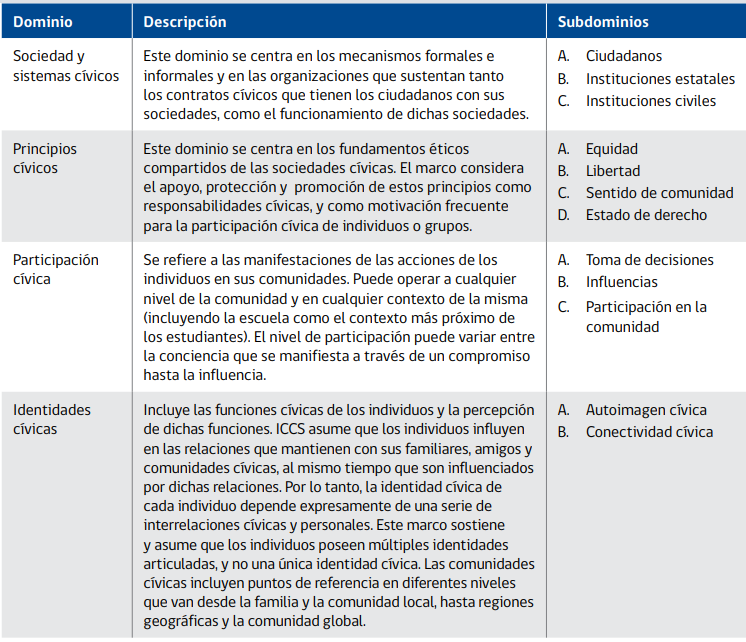
\includegraphics[width=0.8\linewidth,]{images/Contenidos} \end{center}

Cabe destacar, que esta prueba de conocimiento cívico ya ha pasado por tres olas internacionales, a partir de las cuales se ha refinado las características psicométricas de la medición. Esta prueba consta tanto de preguntas de selección múltiple como preguntas abiertas, a continuación, se presenta un ejemplo de pregunta en la cual se miden dominios cognitivos de razonamiento y análisis. Al respecto es importante destacar como esta pregunta requiere tanto de conocimientos políticos, como de habilidades propias del lenguaje como es la interpretación. Al respecto, \citet{schulz_Estudio_2011}, señalan que las preguntas de razonamiento y análisis requieren del uso del lenguaje para interpretar información, relatar, justificar, integrar, generalizar, evaluar, sugerir soluciones o predecir.

\begin{figure}[!ht]

{\centering 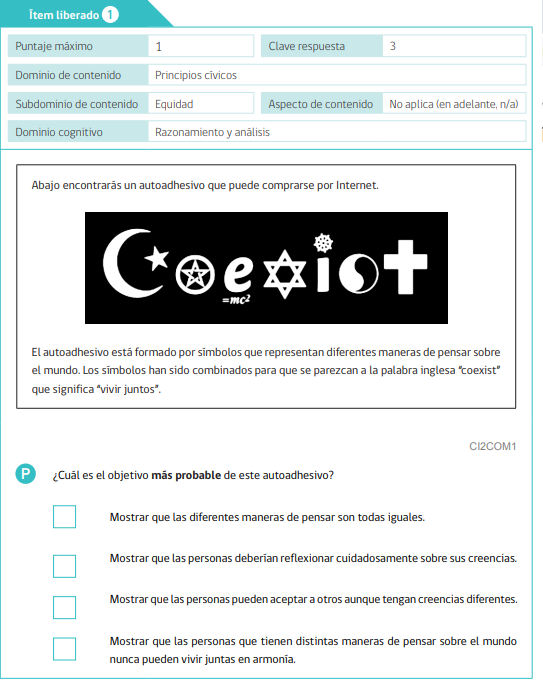
\includegraphics[width=0.8\linewidth,]{images/Pregunta-liberada1} 

}

\caption{pregunta}\label{fig:unnamed-chunk-3}
\end{figure}

En torno a la evidencia levantada sobre el conocimiento cívico de estudiantes medido desde la propuesta de la ICCS, se han señalado fundamentalmente dos conclusiones: primero, el conocimiento cívico posee efectos positivos en valores y conductas democráticas, y segundo, el conocimiento cívico está influido por factores contextuales como la desigualdad social y la socialización escolar.

Debido a sus efectos positivos, el conocimiento cívico y ciudadano es actualmente promovido por diversos agentes a nivel académico, Estatal e internacional. Este conocimiento es sumamente relevante si se considera sus efectos positivos sobre la intención de participación \citep{miranda_Desigualdad_2015}, en un contexto de apatía política y baja participación de estratos bajos y jóvenes \citep{janmaat_Civic_2013, contreras_DIFERENCIAS_2013}. Igualmente, en el contexto de los nuevos movimientos sociales que buscan reivindicar los derechos de distintos grupos tradicionalmente discriminados, el conocimiento cívico ha demostrado estar relacionado con el respeto a los derechos humanos de estos grupos \citep{miranda_Political_2018, caro_Ten_2012}. También, el tener más conocimiento cívico se relaciona con estar en desacuerdo con la corrupción y con la valoración positiva de la democracia como sistema representativo en contraposición a las dictaduras, lo cual, según Hastedt (2016), es fundamental en un contexto de resurgimiento de los gobiernos autoritarios. En suma, el conocimiento cívico puede ayudar a las personas a incorporar los principios democráticos de los derechos humanos.

\hypertarget{conocimiento-civico-y-desigualdad-social}{%
\subsection{Conocimiento civico y desigualdad social}\label{conocimiento-civico-y-desigualdad-social}}

Respecto a las variables que se relacionan con distintos niveles de conocimiento cívico, destacan la influencia del nivel socioeconómico y la influencia de las practicas democráticas en la escuela. Las investigaciones actuales han propuesto que el conocimiento cívico es especialmente influido por variables de origen socioeconómico \citep{ace_Estudio_2017, schulz_Estudio_2011, ferrans_Civic_2017, trevino_Influence_2017}, dando cuenta de lo que se denominará desde este punto, la ``Desigualdad social del conocimiento cívico''. Este efecto del nivel socioeconómico, según la literatura, se debe menos al efecto de la ocupación de los padres que al efecto de variables culturales como la educación de los padres y el número de Libros, dando luces respecto al carácter cultural del fenómeno \citep{castillo_Social_2014}.De este modo, se da cuenta del peso de la socialización familiar en el conocimiento cívico, de modo tal que criarse en un ambiente educado, probablemente con amplio vocabulario, y con acceso a recursos de aprendizaje como lo son los libros, fomenta las habilidades y conocimientos que los jóvenes necesitan para responder la prueba.

Además del efecto de la socialización familiar, otras investigaciones han enfatizado en el efecto producido por variables a nivel escuela como el nivel socioeconómico promedio de la escuela clima más abierto a la discusión y una cultura participativa a nivel escuela son propicios para el conocimiento cívico. En suma, podemos ver que el conocimiento cívico es influido por distintas variables que se relacionan tanto con la socialización familiar como con la escolar, destacando las variables de reproducción cultural.

En consideración de anterior, podemos decir que el conocimiento cívico es bastante explicado por el modelo de recursos, según el cual personas con mayores recursos poseen una mejor disposición a la política \citep{miranda_Desigualdad_2015}. Al explicar esta reproducción fundamentalmente cultural, la teoría de la socialización política familiar destaca dos dimensiones: la actitudinal y la cognitiva. La primera línea teórica destaca la trasmisión de valores e intereses políticos, suponiendo que convivir con padres con un mayor capital cultural conlleva tener conversaciones sobre temas políticos y sociales, que fomentan valores e intereses democráticos en los jóvenes, en contraste con la socialización apolítica de los jóvenes de estratos bajos \citep{gimpel_Cultivating_2003, wasburn_Making_2017}. La segunda, destaca la transmisión de habilidades que son heredadas por la socialización familiar en una cultura académica con lectura temprana y acceso a libros \citep{evans_Scholarly_2015, park_Home_2008}. Esta postura supone que esta cultura académica puede tener un efecto en la socialización política \citep{duarte_influence_2017, boeve-depauw_crossnational_2010}. Por su parte, la disponibilidad de libros en el hogar mejora el rendimiento académico e incrementa las capacidades intelectuales \citep{evans_Scholarly_2015}, mejorando las habilidades para la vida política.

En resumen, las habilidades políticas o el conocimiento civico, son un conjunto de conocimientos y habilidades necesarias para la vida ciudadana, tales como memorización, la interpretación y la evaluación. A partir de la evidencia, se puede sostener que estas habilidades cívicas están muy relacionadas con la socialización política familiar, en la cual influye el origen social. Al explicar esta desigualdad social de las habilidades políticas, la teoría de la socialización recurre tanto a la transmisión de actitudes como de habilidades cognitivas.

\begin{itemize}
\item
  \(H_1\) Existe \emph{desigualdad social del conocimiento civico}, es decir, los estudiantes de familias con mayor nivel socioeconómico poseen un mayor nivel conocimiento cívico.
\item
  \(H_2\) La desigualdad social del conocimiento cívico se explica más por recursos académicos familiares que por el estatus ocupacional. De modo tal que el poseer libros en el hogar posee un mayor efecto sobre el conocimiento cívico que padres con una ocupación de alto estatus.
\end{itemize}

\hypertarget{manejo-del-lenguaje-y-comprensiuxf3n-lectora}{%
\subsection{Manejo del lenguaje y Comprensión lectora}\label{manejo-del-lenguaje-y-comprensiuxf3n-lectora}}

El lenguaje ha sido ampliamente conceptualizado a lo largo del pensamiento humano. Aristoteles, concede al lenguaje un rol elemental cuando lo concibe como la herramienta propia del \emph{zoon politikon}, ya que el lenguaje y la comunicación permite a los humanos discutir y ponerse de acuerdo. Un rol semejante le otorga al lenguaje el filosofó precursor del romanticismo Herder, cuando plantea que esta es la habilidad que da coherencia a la actividad humana, siendo una herramienta que le permite comprender la realidad y reflexionar sobre ella, a partir de conceptualizarla. Desde ambos filósofos, y desde varios otros \citep[ej.][]{echeverria_Ontologia_2011, garcia_LENGUAJE_2013}, el lenguaje es aquello que nos permite relacionarnos como humanos, usar la razón y poder discutir sobre nuestros asuntos para coexistir. Ahora bien, aunque es cierto que el lenguaje es algo propio y por ende transversal en el género humano, existe contundente evidencia para señalar que el manejo del lenguaje es diferenciado según grupos sociales.

Al respecto, el sociólogo de la línea de la reproducción cultural, Basil Berstein, realizo durante algunas décadas un amplio conjunto de experimentos e investigaciones para evaluar el uso del lenguaje en distintas clases sociales. En ellas, \citet{bernstein_CLASES_1985} concluye que los grupos económicamente acomodados y con mayores estudios, heredan a sus hijos un \emph{código sociolingüístico elaborado} del lenguaje, que les permite hacer abstracciones y pensamientos que se separan de la situación contextual en la que se encuentran. Por el contrario, los jóvenes de los barrios obreros heredan gracias al proceso de socialización un \emph{código restringido} el cual esta tendencialmente limitado a referencias contextuales y a situaciones vividas. Cabe destacar, como lo hace \citet{bernstein_Poder_1988}, que los grupos de clases medias y altas también poseen el Código restringido, pero poseen además el código elaborado el cual utilizan en situaciones desafiantes. En suma, puede evidenciarse una desigualdad sociocultural en el manejo del lenguaje que genera capacidades diferenciadas de referenciar ideas fuera de lo vivido cotidianamente, diferencias las cuales explican según el autor la desigualdad de rendimiento académico entre clases sociales, ya que el conocimiento académico se sustenta en el código elaborado, es decir, utiliza ideas fuera de la cotidianidad vivida. En suma, podemos definir al lenguaje como la base de la reflexión y la acción basada en ideas abstractas, el cual puede presentar desarrollos diferenciados socioculturalmente, lo que puede generar desigualdades en ámbitos que requieran de un lenguaje abstracto, como lo puede ser la academia o, desde esta propuesta, la política.

Respecto al manejo del lenguaje, que como vimos es socialmente desigual, y la prueba de conocimiento cívico se han dicho pocas cosas. Entre ellas destaca el aporte de \citet{zhang_Understanding_2015}, quien realiza una critica al instrumento de medición de conocimiento cívico en tanto este posee un lenguaje muy complejo que influye en las respuestas de los estudiantes. Si bien es una critica de validez a considerar, no podemos obviar el hecho de que la política entera esta construida sobre un lenguaje complejo, por lo tanto, el no comprender la prueba por no entender los términos o ser capas de comprender los enunciados planteados, es signo también de no ser capas de comprender esos enunciados fuera del contexto de la prueba. Por ello, complementando lo planteado por \citet{zhang_Understanding_2015} podríamos decir que estas dificultades en el lenguaje de la prueba probablemente son aun mayores para los estudiantes socializados en familias con bajo nivel educativo y menor acceso a recursos como libros.

Un indicador útil para medir la capacidad de los estudiantes de entender distintos discursos y ser capases de comprender ideas abstractas, así como analizarlas, interpretarlas y evaluarlas, es la comprensión lectora. La comprensión lectora implica la medición de la capacidad del estudiante, no solo de decodificar el texto, sino de comprender y analizar la relación entre las distintas partes de los textos, para posteriormente realizar ejercicios mentales más complejos como los son la síntesis, la interpretación la evaluación \citep{ace_Informe_2018}. Si bien otras habilidades del manejo del lenguaje como la comprensión auditiva y la expresión escrita u oral son habilidades fundamentales para la vida política, poseen la dificultad de que es sumamente difícil medirlas de modo estandarizado. No obstante, no incorporarlas no es tan problemático considerando la amplia relación que hay entre comprender la lectura y estas otras habilidades. Para trabajar con esta variable se utilizará la prueba SIMCE, la cual, justamente busca medir los logros de aprendizaje de los estudiantes chilenos en torno a las habilidades lectoras.

Según \citet{barahonau_Factores_2014} existe un consenso en que los factores asociados al desempeño académico en lenguaje pueden tener su origen en dos grandes ámbitos: en los determinantes personales y en los determinantes sociales. Así, una de las variables fundamentales para explicar el rendimiento en lenguaje es el nivel socioeconómico según se plantea en el informe Coleman \citep{marques_Apuntes_2016}. No obstante, no todo es reproducción social, pues como plantean \citet{lara_mirada_2010}, las practicas docentes pueden tener un efecto positivo, por ejemplo, discutir la materia en clases es positivo para el rendimiento en comprensión lectora. Además de la participación en clases, el interés sobre la materia es un factor fundamental para su aprendizaje \citep{lozano_Relacion_2000}.

\hypertarget{suxedntesis-e-hipuxf3tesis.}{%
\section{Síntesis e hipótesis.}\label{suxedntesis-e-hipuxf3tesis.}}

La política y el lenguaje están altamente relacionados, de modo tal que mejores habilidades lingüísticas fomentan mejores habilidades políticas. Definimos la política como un espacio de resolución de problemas, de conflicto social y de cohesión social. Por su parte, el lenguaje fue definido como una herramienta del pensamiento humano, que permite articular individuo y sociedad, a la vez que posibilita la crítica. No obstante, como evidenciamos con las propuestas teóricas de la teoría de la reproducción cultural, las habilidades para el manejo del lenguaje se encuentran desigualmente distribuidas en la población.

En vista de lo anterior, proponemos que la reproducción intergeneracional de la desigualdad política, evidenciada en el campo de la educación cívica, puede ser explicada en cuanto a su mecanismo causal por el que opera incorporando el lenguaje como una habilidad que se transmite intergeneracionalmente y que otorga ventajas para incorporarse en la política.

En suma, el manejo del lenguaje es una habilidad que permite la reflexión, la cual es fundamental para actividades que requieren de abstracción como lo es la académica y la política. Este manejo, es adecuadamente medido por la prueba de comprensión lectora que evalúa habilidades como la comprensión, el análisis y la interpretación. Según la evidencia, el manejo del lenguaje es influido por variables socioeconómicas, por variables individuales; como el interés en la materia y por características de la escuela; como una educación participativa. Además considerando la desigualdad social en el manejo del lenguaje y la complejidad del lenguaje de le prueba de conocimiento cívico, es esperable que parte de la desigualdad social del conocimiento civico se deba a las diferencias en torno al manejo del lenguaje.

En vista de las reflexiones y evidencias anteriores se proponen las siguientes hipótesis.

\begin{itemize}
\tightlist
\item
  \(H_2\) El manejo del lenguaje posee un efecto positivo sobre el conocimiento cívico del estudiante.
\item
  \(H_3\) El manejo del lenguaje media parcialmente la relación del estatus ocupacional y educacional de los padres sobre el conocimiento cívico del estudiante.
\item
  \(H_4\) El manejo del lenguaje media totalmente la relación entre cantidad de libros en el hogar y el conocimiento cívico del estudiante.
\end{itemize}

\begin{figure}[!ht]

{\centering 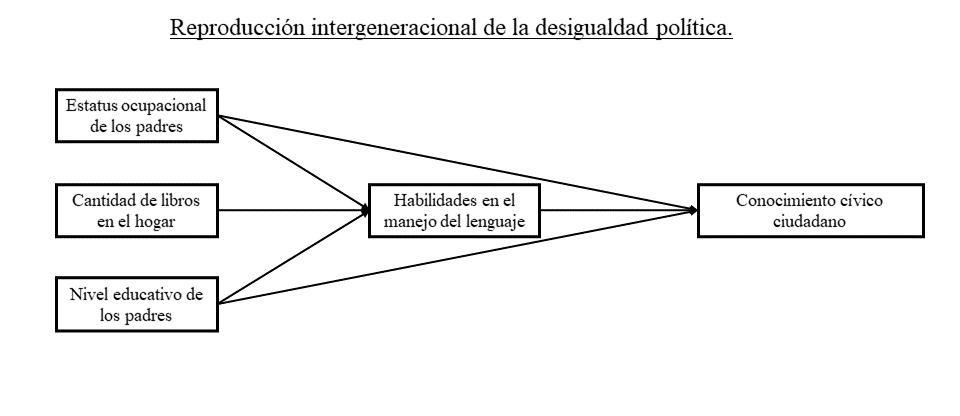
\includegraphics[width=0.95\linewidth,]{images/modelo} 

}

\caption{Modelo Teorico}\label{fig:unnamed-chunk-4}
\end{figure}

Junto con lo anterior, y considerando la capacidad positiva del colegio de mejorar la comprensión lectora de sus estudiante mediante buenas practicas como la discusión en clase y la motivación de sus estudiantes, se propone que el colegio puede fomentar un manejo del lenguaje que supere el efecto de la familia, lo cual podría moderar las desigualdades sociales del conocimiento cívico.

\begin{itemize}
\tightlist
\item
  \(H_4\) El manejo del lenguaje es capas de moderar el efecto del nivel socioeconómico sobre el conocimiento cívico.
\end{itemize}

\hypertarget{metodologuxeda}{%
\chapter{Metodología}\label{metodologuxeda}}

\hypertarget{datos}{%
\section{Datos}\label{datos}}

\hypertarget{iccs}{%
\subsection{ICCS}\label{iccs}}

Para abordar la pregunta de investigación se trabajará con la base de datos de la encuesta internacional de conocimiento cívico (ICCS) en su tercera versión (2016). La ICCS es una encuesta enfocada en el estudio longitudinal del conocimiento cívico y las actitudes democráticas en estudiantes de octavo grado de 24 países. Dieciséis de esos países son de Europa, cinco de América Latina y tres de Asia, representados por 94.000 estudiantes y 37.000 profesores de 3.800 colegios \citep{schulz_ICCS_2016}. Junto con una estrecha colaboración entre la IEA y los centros de estudios de cada país, los encargados de la elaboración de los datos fueron El Consejo Australiano para la Investigación Educativa (ACER) en Melbourne y el Laboratorio di Pedagogia Sperimentale (LPS) en la Universidad Roma Tre \citep{iea_International_2016}. La muestra de estudiantes posee un diseño estratificado de dos etapas, eligiendo escuelas al azar en un país y aulas al azar en una escuela, de tal modo que cada país tenga aproximadamente 150 escuelas y entre 3000 y 45000 estudiantes. La muestra de chile, con trabajo de campo en el 2015, incorporo colegios elegidos aleatoriamente, y representativos de distintas dependencias y regiones, tanto de sectores rurales como urbanos. De las escuelas seleccionadas aleatoriamente el 85\% acepto participar, y dentro de las escuelas participantes, el 85\% de los estudiantes acepto participar. En total, participaron 5.081 estudiantes de 178 establecimientos según señala la agencia de calidad de la educación \citep{ace_Informe_2018a}.

\hypertarget{simce}{%
\subsection{SIMCE}\label{simce}}

Adicionalmente se utilizaron los datos Simce del 2015, prueba censal que fue aplicada a los mismos estudiantes participantes del estudio de la ICCS, lo cual permite agregar estas bases de datos, logrando tener las variables de ambos estudios para cada estudiante de la muestra del ICCS. El Simce evalúa los logros de aprendizaje en las asignaturas de Lenguaje y Comunicación (Comprensión Lectura y Escritura); Matemática; Ciencias Naturales; Historia, Geografía y Ciencias Sociales e Inglés. En esta ocasión, hemos utilizado los datos de la prueba Simce de lenguaje y comunicación, más específicamente, de comprensión lectora. El estudio Simce, al igual que el ICCS, trabaja con el modelo de medición de ITR (Teoria de respuesta al ítem). "En particular {[}el Simce trabaja con{]} el modelo IRT de tres parámetros, {[}el cual{]} permite estimar la habilidad de un estudiante, basándose en la probabilidad de respuesta correcta según tres características propias de las preguntas: dificultad, discriminación y azar \citep{ace_Informe_2018}. Los procesos de aplicación de los instrumentos (pruebas y cuestionarios10) se llevan a cabo en función de instrucciones, manuales y protocolos de actuación que se basan en los criterios de estandarización internacional \citep{aera_Report_2011}.

Respecto al tipo de preguntas, estas son de opción múltiple, pues este formato permite reportar información de la mayoría de los constructos a evaluar en forma efectiva y eficiente, asegurando validez, confiabilidad y objetividad del instrumento en su totalidad \citep{rupp_Handbook_2008}. En miras de este objetivo de la validez del instrumento, se realizan desde el año anterior a la aplicación pruebas piloto, las cuales son analizadas cualitativa y cuantitativamente para construir los indicadores más adecuados posibles. En suma, el Simce realiza una Logística de preparación que implica un gran gasto de recursos con el objetivo de reducir al máximo el error de medida.

\hypertarget{variables}{%
\section{Variables}\label{variables}}

\hypertarget{prueba-de-conocimiento-cuxedvico-y-ciudadano}{%
\subsection{Prueba de conocimiento cívico y ciudadano}\label{prueba-de-conocimiento-cuxedvico-y-ciudadano}}

La prueba de conocimiento cívico de la ICCS, tiene como objetivo evaluar los conocimientos necesarios para comprender y valorar la vida en sociedad y las formas de organización democrática, la capacidad de razonar acerca de las instituciones, eventos, acciones y procesos que se desarrollan en sus comunidades y la habilidad de desarrollar y justificar opiniones y visiones sobre estos elementos \citep{schulz_Initial_2010}. Los ítems de prueba requerían que los estudiantes aplicaran los procesos cognitivos al contenido cívico y de ciudadanía como se describe en el marco de evaluación del reporte técnico \citep{schulz_ICCS_2016}. Más específicamente, la prueba de conocimiento Cívico y ciudadano mide:

\begin{itemize}
\tightlist
\item
  \emph{Dominios de contenido}

  \begin{itemize}
  \tightlist
  \item
    Sociedad y sistemas cívicos
  \item
    principios cívicos
  \item
    Participación cívica
  \item
    Identidades cívicas
  \end{itemize}
\item
  \emph{Dominios cognitivos}

  \begin{itemize}
  \tightlist
  \item
    conocimiento memorización
  \item
    Razonamiento y aplicación
  \end{itemize}
\end{itemize}

Se utilizaron dos formatos de ítems: 79 de 88 ítems de la prueba son de opción múltiple con cuatro opciones de respuesta, como se puede ver en los ejemplos de los Anexos; los nueve ítems restantes fueron de respuesta construida para los cuales los estudiantes debían escribir entre una y tres oraciones. Para calcular los puntajes de cada estudiante, se parte de una media de 500 puntos, considerando una desviación estándar de 100 puntos, y según esta métrica se calculan 5 posibles resultados para cada estudiante. El que sean 5 resultados refleja el error y la incertidumbre propia de la medición de constructos complejos, al respecto se ha decidido trabajar con la primera estimación de puntaje. Según el reporte técnico \citep{schulz_ICCS_2016}, se utilizó la teoría de respuesta al ítem. Para escalar los datos de prueba de ICCS 2016, los autores recurrieron al paquete de software de escalado ACER ConQuest, Versión 4. Posteriormente se realizaron diversas pruebas de validez, confiabilidad y equivalencia para comprobar que el conocimiento cívico es un constructo unidimensional, continuo y fiable.
Además de las evaluaciones de fiabilidad, invarianza, equivalencia y validez realizadas por los centros de investigación designados por la IEA en el marco de la ICCS, otras agencias han evaluado la calidad de los cuestionarios. Así, por ejemplo, la agencia nacional de educación, evaluar el sesgo de deseabilidad social, concluyendo que la prueba no presenta problemas mayores de deseabilidad, y que estos se concentran en los aspectos de preguntas de actitudes y opiniones (Mineduc, 2019).

A continuación, se presenta una tabla con distintos rangos de puntaje y distintas capacidades que son asociadas a este puntaje. Como puede verse seria optimo que los jóvenes alcancen puntajes de conocimiento cívico superiores a 563 puntos.

\begin{figure}[!ht]

{\centering 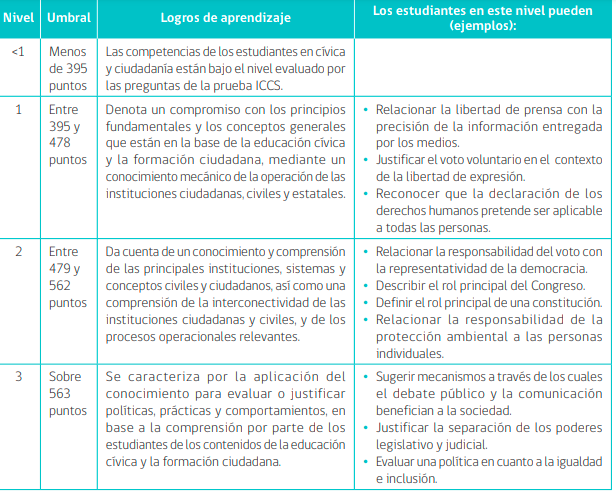
\includegraphics[width=0.8\linewidth,]{images/puntajesdecorteiccs} 

}

\caption{rangos iccs}\label{fig:unnamed-chunk-5}
\end{figure}

\hypertarget{prueba-de-comprensiuxf3n-lectora}{%
\subsection{Prueba de comprensión lectora}\label{prueba-de-comprensiuxf3n-lectora}}

La comprensión lectora busca evaluar a los estudiantes en su capacidad de manejo del lenguaje y la comunicación. Específicamente, la prueba de lenguaje evalúa las siguientes actividades.

\begin{itemize}
\tightlist
\item
  Localizar información

  \begin{itemize}
  \tightlist
  \item
    Identificar
  \item
    Discriminar
  \item
    Extraer
  \end{itemize}
\item
  Interpretar

  \begin{itemize}
  \tightlist
  \item
    Inferir
  \item
    Interpretar lenguaje denotativo
  \item
    Reconocer relaciones causales
  \end{itemize}
\item
  Reflexionar

  \begin{itemize}
  \tightlist
  \item
    Contrastar con conocimientos previos
  \item
    Evaluar críticamente aspecto de contenido y formato
  \end{itemize}
\end{itemize}

Así, como puede apreciarse, para un buen puntaje en comprensión lectora, no solo se requiere la capacidad de decodificar el significado de las palabras, sino que se requiere un manejo del lenguaje a un nivel de razonamiento. Como ya se comentó, el proceso de elaboración y aplicación de la prueba tiene el objetivo de disminuir al mínimo variables externas al manejo del lenguaje que pudieran afectar la medición. Para evaluar las propiedades psicométricas de esta prueba, los encargados de la prueba Simce realizaron análisis en base a lineamientos internacionales \citep{aera_Report_2011}. En base a los análisis realizados por el equipo técnico \citep{ace_Informe_2018}, podemos decir que la prueba de comprensión lectora es unidimensional (i.e El AFC indica un solo factor), posee independencia local (i.e estudiantes de un mismo rendimiento no presentan dificultades para determinada pregunta por factores externos) y motricidad creciente (i.e es un constructo continuo donde la probabilidad de responder correctamente un ítem aumenta progresivamente en estudiantes de mayor rendimiento).

\begin{figure}[!ht]

{\centering 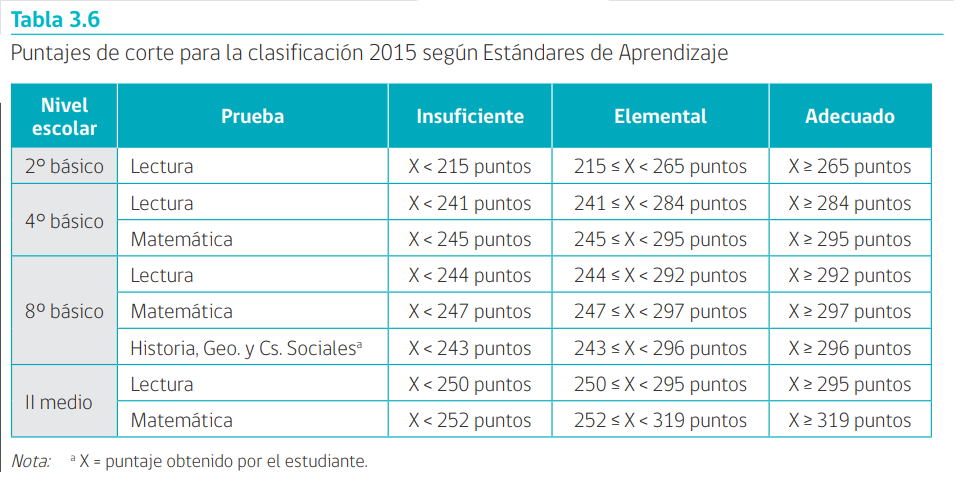
\includegraphics[width=0.8\linewidth,]{images/Rangos-puntaje-simce} 

}

\caption{rangossimce}\label{fig:unnamed-chunk-6}
\end{figure}

\hypertarget{estatus-socioeconuxf3mico-del-estudiante-y-del-colegio.}{%
\subsection{Estatus socioeconómico del estudiante y del colegio.}\label{estatus-socioeconuxf3mico-del-estudiante-y-del-colegio.}}

Para trabajar la medicación del estatus socieconómico del colegio, se trabajara con tres variables, el estatus ocupacional más alto entre los padres, el nivel educativo más alto de los padres y la cantidad de libros en le hogar. Para simplificar los cálculos a realizar, las dos ultimas variables sera dicotomizadas de tal modo que representen, tener un padre con educación universitaria y poseer más de 100 libros en el hogar respectivamente. Dicotomizar las variables permitira disminuir la cantidada de parametros a estimar y la existencia de categorias con muy pocas respuestas en las escuelas las cuale sestan altamente segregadas socioeconomicamente. Estas variables serán utilizadas para trabajar la mediación.

Para trabajar la moderación del efecto del nivel socioeconómico de los estudiantes se utilizará el Índice nacional de antecedentes socioeconómicos el cual es elaborado por el equipo de la ecuesta ICCS. Este índice es elaborado como un puntaje factorial que representa una variable latente relacionada con el mayor nivel ocupacional entre los padres, el mayor nivel educativo entre los padres y la cantidad de libros declarados en el hogar. Para evaluar el contexto socioeconómico del establecimiento educativo, se trabajará con el promedio por colegio del Índice nacional de antecedentes socioeconómicos.

\hypertarget{interuxe9s-poluxedtico}{%
\subsection{Interés político}\label{interuxe9s-poluxedtico}}

Para medir el interés político los estudiantes se utilizará la pregunta creada por la encuesta internacional ICCS. En este ítem se le pregunta al estudiante ¿Qué tan interesado está en temas políticos y sociales? (Muy interesado/ Bastante interesado / No muy interesado / No me interesa en absoluto). Para simplificar el análisis se ha recodificado esta pregunta de tal modo que las dos primeras alternativas se resumen en ``Interesado en la politica'' y las últimas dos en ``No interesado en la politica''. Cabe destacar que, para el análisis de mediación, se utilizó la variable original de 4 categorías centrada al promedio de la escuela.

\hypertarget{variables-de-control}{%
\subsection{Variables de control}\label{variables-de-control}}

Como variables de control, será incluida la calidad de la discusión en el aula, ya que este es un indicador que ha sido consistentemente señalado como relevante por la evidencia, esta variable de nivel dos corresponde al promedio de los indicadores relacionados con las preguntas de clima en el aula.

\hypertarget{muxe9todos}{%
\section{Métodos}\label{muxe9todos}}

Respecto al método, este estudio trabajara desde un enfoque cuantitativo transversal. El uso de las herramientas cuantitativas es fundamental para despejar las dudas planteadas en este artículo, puesto que la cuantificación, como medición de lo social \citep{canales_METODOLOGIAS_2006}, nos permitirá contrastar que variable posee una mejor capacidad mediadora de la reproducción de la desigualdad política, la comprensión lectora o el interés político. A continuación, se hace una exposición de las técnicas con las que se trabajara y se explicara por que son indispensables para abordar la temática.

El centro del trabajo utilizara estadística multivariada, más particularmente, regresiones lineales. Las regresiones lineales según Hayes poseen la intención evaluar la capacidad predictiva de una variable sobre otra. Para representar la relación gráfica y numéricamente, se busca restimar una línea que represente la relación entre una variable independiente y una dependiente. Esta línea se superpone a un gráfico de dispersión en el cual cada caso s situado en una posición según su valor en el eje x y el eje ``y''. De este modo, cuando no hay relación se forma una nube dispersa, mientras que más es la relación los puntos se ajustan más a una línea. La regresión nos permite encontrar la línea que mejor representa la relación .Esta línea en un plano cartesiano nos permite tener conclusiones del tipo ``mientras más se tiene de esta variable más se tiene de esta otra''. Para llegar a estimar esa línea que representa mejor la relación se utiliza la técnica de mínimos cuadrados, la cual es un proceso iterativo donde a partir de probar múltiples rectas, se evalúa cual de ellas genera la menor cantidad de residuos. Los residuos corresponden a la varianza de la dependiente que no es explicada por la independiente. Si dos variables están completamente relacionadas no habrá residuos, y la línea pasará por cada uno de los puntos del gráfico. Matemáticamente, esto implica que el valor de los casos en el plano restado a el valor predicho es 0. Se realiza un calculo que busca encontrar la recta que genera el mínimo, de residuos y por ende representa mejor la relación, que se supone lineal.

Las relaciones pueden ser positivas o negativas. Cuando una relación es positiva se ve que la línea que mejor representa la relación parte al comienzo del grafico en la izquierda en un valor menor y que aumenta en tanto avanza a la derecha. Una relación negativa por el contrario implica que a mayor valor de x menor valor de y.

Los parámetros entregados por la regresión son, p de significación, betas que representan la relación, r2 que representan la fuerza de la relación y un intercepto, el cual corresponde al promedio en un modelo sin predictores y aumenta o disminuye según se incline la línea de predicción. Por ende, el intercepto puede ser interpretado como el corte con le eje y cuando la variable dependiente esta en 0, lo cual no siempre tiene una aplicación directa.

Las ventajas de las regresiones son múltiples. En primer lugar, como medida de relación cumple con las exigencias señalada por la metodología. Posee un valor p que nos permite evaluar si es posible extrapolar las conclusiones al universo. Este valor p representa la posibilidad de que la pendiente sea efectivamente distinta a 0, es decir, la posibilidad de que no exista relación. Además, siguiendo los consejos de Cohen, las regresiones entregan un valor que indica la fuerza de la relación lo cual es fundamental para comprender la magnitud de los fenómenos que estamos evaluando.

Una segunda ventaja de las regresiones líneas para nuestro trabajo es que permiten realizar control estadístico. El control estadístico es un proceso complejo por el cual mediante la parcialización de los efectos se puede despejar los efectos comunes de dos variables, para evaluar cual es efectivamente la que posee una influencia sobre la dependiente. De este modo, siguiendo con nuestras hipótesis, el efecto que es generado inicialmente por el nivel socioeconómico debería poder ser controlado por el efecto del manejo del lenguaje, por que en ultima instancia las diferencias deben al mejor manejo del lenguaje en los niveles socioeconómico más altos. Otra forma de entender el control estadístico es considerar los efectos controlados como el efecto de una variable cuando la otra esta constantemente en 0.

El control estadístico se logra a partir del proceso de parcialización el cual corresponde a explicar una independiente por otra independiente, y eliminar todo aquello que es explicado (varianza compartida) utilizando los residuos de esa regresión como variable independiente.

Se trabajará con técnicas de regresión multinivel, ya que estas son indispensables al estudiar muestras jerárquicas de colegios. Las regresiones multinivel, a diferencia de las regresiones normales, asumen que los estudiantes de un mismo establecimiento compartirán características debido al contexto común. Si se trabajara con regresiones lineales de un solo nivel, se rompería el supuesto de independencia de los casos en la muestra, ya que los casos están relacionados entre sí al pertenecer a los mismos establecimientos. Esta metodología también nos permite evaluar el efecto de características de la escuela, como lo son el NSE promedio o la percepción promedio de apertura a la discusión. Más específicamente, dentro del trabajo con regresiones multinivel, se trabajará con relaciones pendientes aleatorias, mediación multinivel e interacciones entre niveles.

Para entender el concepto de multinivel y su operación estadística es necesario primero comprender la idea de varianza entre y dentro. Pensemos en comprensión lectora. Es sabido que existen colegios que poseen una mejor comprensión lectora que otros. Este efecto no se debe particularmente a que cada uno de los niños, sino que se puede deber a que el colegio posee una mejor educción o a que es más selectivo. De este modo se puede ver que hay varianza entre los estudiantes que corresponde a la varianza entre los colegios. Es el efecto de pertenecer a un mejor colegio que otro. Por otro lado, además de esas diferencias entre colegios hay diferencias dentro de los colegios. Entre estudiantes de un liceo de mal desempeño, existen estudiantes mejores que otros y algunos que pueden sobresalir. En alguna medida, se puede esperar que estas diferencias dentro de las escuelas sean producto del esfuerzo del niño o de los apoyos y ventajas que les ofrecen sus padres.

Con esa distinción conceptual en mente, veamos que hacen las regresiones multinivel. Para ello es necesario comprender que estas regresiones consideran los grupos en los cuales esta cada sujeto, en este caso las escuelas. Estadísticamente diferencian los residuos de la varianza, en residuos entre colegios y residuos dentro de los colegios. Cuando una variable a nivel escuela como la calidad de los profesores afecta la variable dependiente, esta reducirá los residuos entre colegios. Por su parte, cuando se tiene una variable individual que afecta las diferencias entre los niños, como poseer profesores particulares, esto disminuirá la varianza dentro de las escuelas.

Para la existencia de los residuos diferenciados, es necesaria la estimación de dos tipos de líneas de regresión. La primera es una pendiente general que representa la relación a nivel 2. El segundo tipo de línea, son las pendientes en cada grupo. Esta diferencia permite la variación de los parámetros entre los grupos. De este modo, se pueden agregar dos parámetros muy interesantes. Un intercepto aleatorio y una pendiente aleatoria. El termino aleatorio no refiere a que es azaroso, sino que varia entre grupos.\\
La variación de los intercepto nos indica cuando dieren los intercepto entre los grupos. El intercepto aleatorio nos puede indicar que en algunos establecimientos el nivel de conocimiento cívico (variable y) es mayor ante el valor mínimo de manejo del lenguaje (variable x)
Las pendientes aleatorias sirven para evaluar como varia la pendiente de una relación en distintos contextos, para este trabajo se calculará la variación de la pendiente de la relación entre conocimiento cívico y comprensión lectora.

La medición multinivel permite evaluar una cadena causal considerando la estructura jerárquica de los datos. Para comprender esta metodología, es necesario entender que una medicación corresponde al fenómeno según el cual una variable ``X'', explica una variable ``Y'', por medio de ``M'', de tal modo que ``X'' genera ``M'' y M genera ``Y'' \citep{mathieu_framework_2007}. Al igual que en una mediación de un solo nivel, es requisito para comprobar la mediación multinivel, que ``X'' sea capaz de explicar tanto ``M'' como ``Y'', y que, además, M sea capaz de explicar ``Y'', controlando, en alguna medida el efecto de ``X'' \citep{baron_moderator_1986}. Existen distintos tipos de análisis de mediación cuando se trabaja con lógicas multinivel. Se puede hablar de mediaciones intra-niveles que solo involucran una mediación dentro del Nivel 1 o Nivel 2, y también se puede hablar de meso-mediaciones, en las cuales la mediación pasa de un nivel a otro \citep{mathieu_framework_2007}. En nuestro caso, contamos con una mediación intra-nivel, ya que todas las variables involucradas en la mediación son de nivel 1, aunque sea relevante considerar y controlar por características de Nivel 2 ya que los datos están anidados. En nuestro caso, queremos evaluar la capacidad de la comprensión lectora de mediar la relación entre NSE y conocimiento cívico, por ende, debemos evaluar la capacidad explicativa del NSE sobre la comprensión lectora y el conocimiento cívico (CC), y posteriormente, ver la capacidad del manejo del lenguaje de controlar el efecto del NSE sobre CC.

Considerando las recomendaciones de \citep{zhang_Testing_2009} para cuando todas las variables del proceso de mediación se encuentran en el primer nivel, es fundamental, para evitar confusiones de los efectos producidas por la estructura jerárquica de la muestra, evaluar las relaciones en ambos niveles, es decir, un efecto de mediación intragrupo y otro entre grupos, para ello se deben realizar centrados en las medias de los grupos, según concluyeron los investigadores a partir de pruebas de simulación Montecarlo.

Esta propuesta si bien será utilizada y es muy enriquecedora metodológicamente, posee dos limitaciones que es necesario resolver para poder trabajar rigurosamente nuestras hipótesis. En primer lugar, esta forma de trabajar las relaciones multinivel no permite saber si el efecto indirecto es significativo, como Sobel señala necesario. Por ello para subsanar esta falencia se utilizará la prueba de Sobel. En segundo lugar, esta perspectiva tampoco permite abordar los tamaños de efecto, por lo cual se considera necesario incluir el efecto mediado en términos de R2, para lo cual se recurrirá a la estimación de Bryk \& Raudenbusch (1992).

A continuación, se expone el calculo que a realizar para probar la mediación multinivel. En general el modelo señala que el Conocimiento cívico es explicado por la comprensión lectora, la cual a su vez se debe a los recursos de la familia. El modelo también calcula los efectos directos e indirectos de los recursos de la familia sobre el conocimiento cívico. Las siguientes formulas no contienen todos los controles señalados.

\begin{enumerate}
\def\labelenumi{\alph{enumi})}
\tightlist
\item
  \emph{Influencia de los recursos familiares en el lenguaje}
\end{enumerate}

\begin{equation}
\text{C.Lectora}= i_1 +\gamma_{10}\text{Ocupación}_{ij} + \gamma_{20}\text{Universitarios}_{ij}+ \gamma_{30}\text{Libros}_{ij}+u_{0j}+r_{ij}
\end{equation}

\begin{enumerate}
\def\labelenumi{\alph{enumi})}
\setcounter{enumi}{1}
\tightlist
\item
  \emph{Influencia directa de los recursos familiares en lo cívico}
\end{enumerate}

\begin{equation}
\text{C.Civico}= i_2+\gamma_{40}\text{Ocupación}_{ij} + \gamma_{50}\text{Universitarios}_{ij}+ \gamma_{60}\text{Libros}_{ij}+u_{0j}+r_{ij}
\end{equation}

\begin{enumerate}
\def\labelenumi{\alph{enumi})}
\setcounter{enumi}{2}
\tightlist
\item
  \emph{Influencia del lenguaje e influencia controlada de los recursos familiares en lo cívico}
\end{enumerate}

\begin{equation}
\text{C.Civico}= i_+\gamma_{70}\text{C.Lectora}_{ij}+\gamma_{70}\text{Ocupación}_{ij} + \gamma_{80}\text{Universitarios}_{ij}+ \gamma_{90}\text{Libros}_{ij}+u_{0j}+r_{ij}
\end{equation}

\begin{itemize}
\item
  Efectos indirectos de recursos familiares sobre conocimiento civico

  \begin{itemize}
  \item
    Ocupación de los padres = \(\gamma_{10}\times\gamma_{70}\)
  \item
    Padres Universitarios = \(\gamma_{20}\times\gamma_{80}\)
  \item
    Libros en el hogar = \(\gamma_{30}\times\gamma_{90}\)
  \end{itemize}
\end{itemize}

En suma, se evaluará la medicación de la comprensión lectora sobre la relación entre NSE y conocimiento Cívico, evaluando la relación a nivel dos y a nivel uno, incorporando centrados a la media del grupo. Se espera que el efecto de NSE sobre CC disminuya en buena medida al incluir el control de la comprensión lectora. además, se espera que la disminución del efecto por control sea mayor al incluir la variable comprensión lectora que interés político.

En términos de interacciones entre niveles, evaluaremos la capacidad de la comprensión lectora del estudiante de moderar el efecto negativo sobre el conocimiento cívico que se debería de pertenecer a un establecimiento de bajo NSE promedio. Siguiendo las buenas prácticas para interacciones multinivel propuestas por \citep{aguinis_BestPractice_2013}, se centraron las variables según el promedio de la escuela, con la intención de despejar debidamente el componente individual de la varianza.

\hypertarget{software}{%
\subsection{Software}\label{software}}

El software de análisis estadístico utilizado fue R (versión 4.02) y la plataforma de edición Github. Para los análisis multinivel recurrimos al paquete lme4, en su versión 1.1-23 \citep{bates_Package_2020}.

Además, siguiendo los lineamientos de la ciencia abierta, este trabajo está en un repositorio para facilitar tanto su acceso como su reproductibilidad. El lector de este seminario esta cordialmente invitado a visitar la \href{https://franciscomeneses.github.io/Seminario/docs/index.html}{página web del proyecto} en la que se puede revisar tanto el articulo como los análisis. Igualmente, si el lector desea reproducir los análisis para verificar su veracidad, puede descartar el proyecto desde el \href{https://github.com/franciscomeneses/Seminario}{repositorio de Github}. Para facilitar la comprensión del orden de los archivos, estos se han ordenado según el esquema \href{https://juancarloscastillo.github.io/ipo/}{IPO}, propuesto por Castillo (2020)

\hypertarget{anuxe1lisis}{%
\chapter{Análisis}\label{anuxe1lisis}}

A continuación, se presentan análisis uni y bivariados para las variables más importantes del estudio. De este modo buscamos aproximarnos a la realidad del país para sacar mejores conclusiones en torno a los modelos. De este modo, podremos comprender los actuales niveles de conocimiento cívico y comprensión lectora de nuestros estudiantes. Para los análisis descriptivos, bivariados y multivariados, se utilizan los puntos de corte del conocimiento cívico y de la comprensión lectora señalados respectivamente por el Mineduc y los representantes de la IEA. Los puntos de corte ayudaran a comprender la magnitud de las diferencias y las reales implicancias de la temática.

\hypertarget{anuxe1lisis-descriptivo}{%
\section{Análisis descriptivo}\label{anuxe1lisis-descriptivo}}

El presente gráfico presenta la distribución del conocimiento cívico en los estudiantes chilenos de octavo básico del 2015. Junto a la distribución se expone el porcentaje de estudiantes que se encuentra en cada nivel del conocimiento cívico. Como se puede ver en la imagen casi un 15\% de los estudiantes se encuentra por debajo del nivel que pretende medir la prueba de la ICCS, lo cual es un dato bastante preocupante. Seguidamente un cuarto de los estudiantes posee conocimientos cívicos y algún compromiso con valores democráticos, pero no comprende el funcionamiento de las principales instituciones. Un tercio de los estudiantes si comprende los conceptos más relevantes y es capaz de comprender la interacción de las distintas instituciones cívicas y ciudadanas en procesos relevantes, pero no es capaz de aplicar estos conocimientos para evaluar situaciones concretas. Finalmente, la cuarta parte de los estudiantes alcanzan el máximo nivel señalado por la ICCS, denotando ser capases de aplicar estos conocimientos para evaluar o justificar situaciones concretas. Cabe destacar que el promedio de los estudiantes bordea los 500 puntos, estando en el nivel de compresión, además el puntaje mínimo es 232,1 y el puntaje máximo es 782,7.

\begin{figure}[!ht]

{\centering 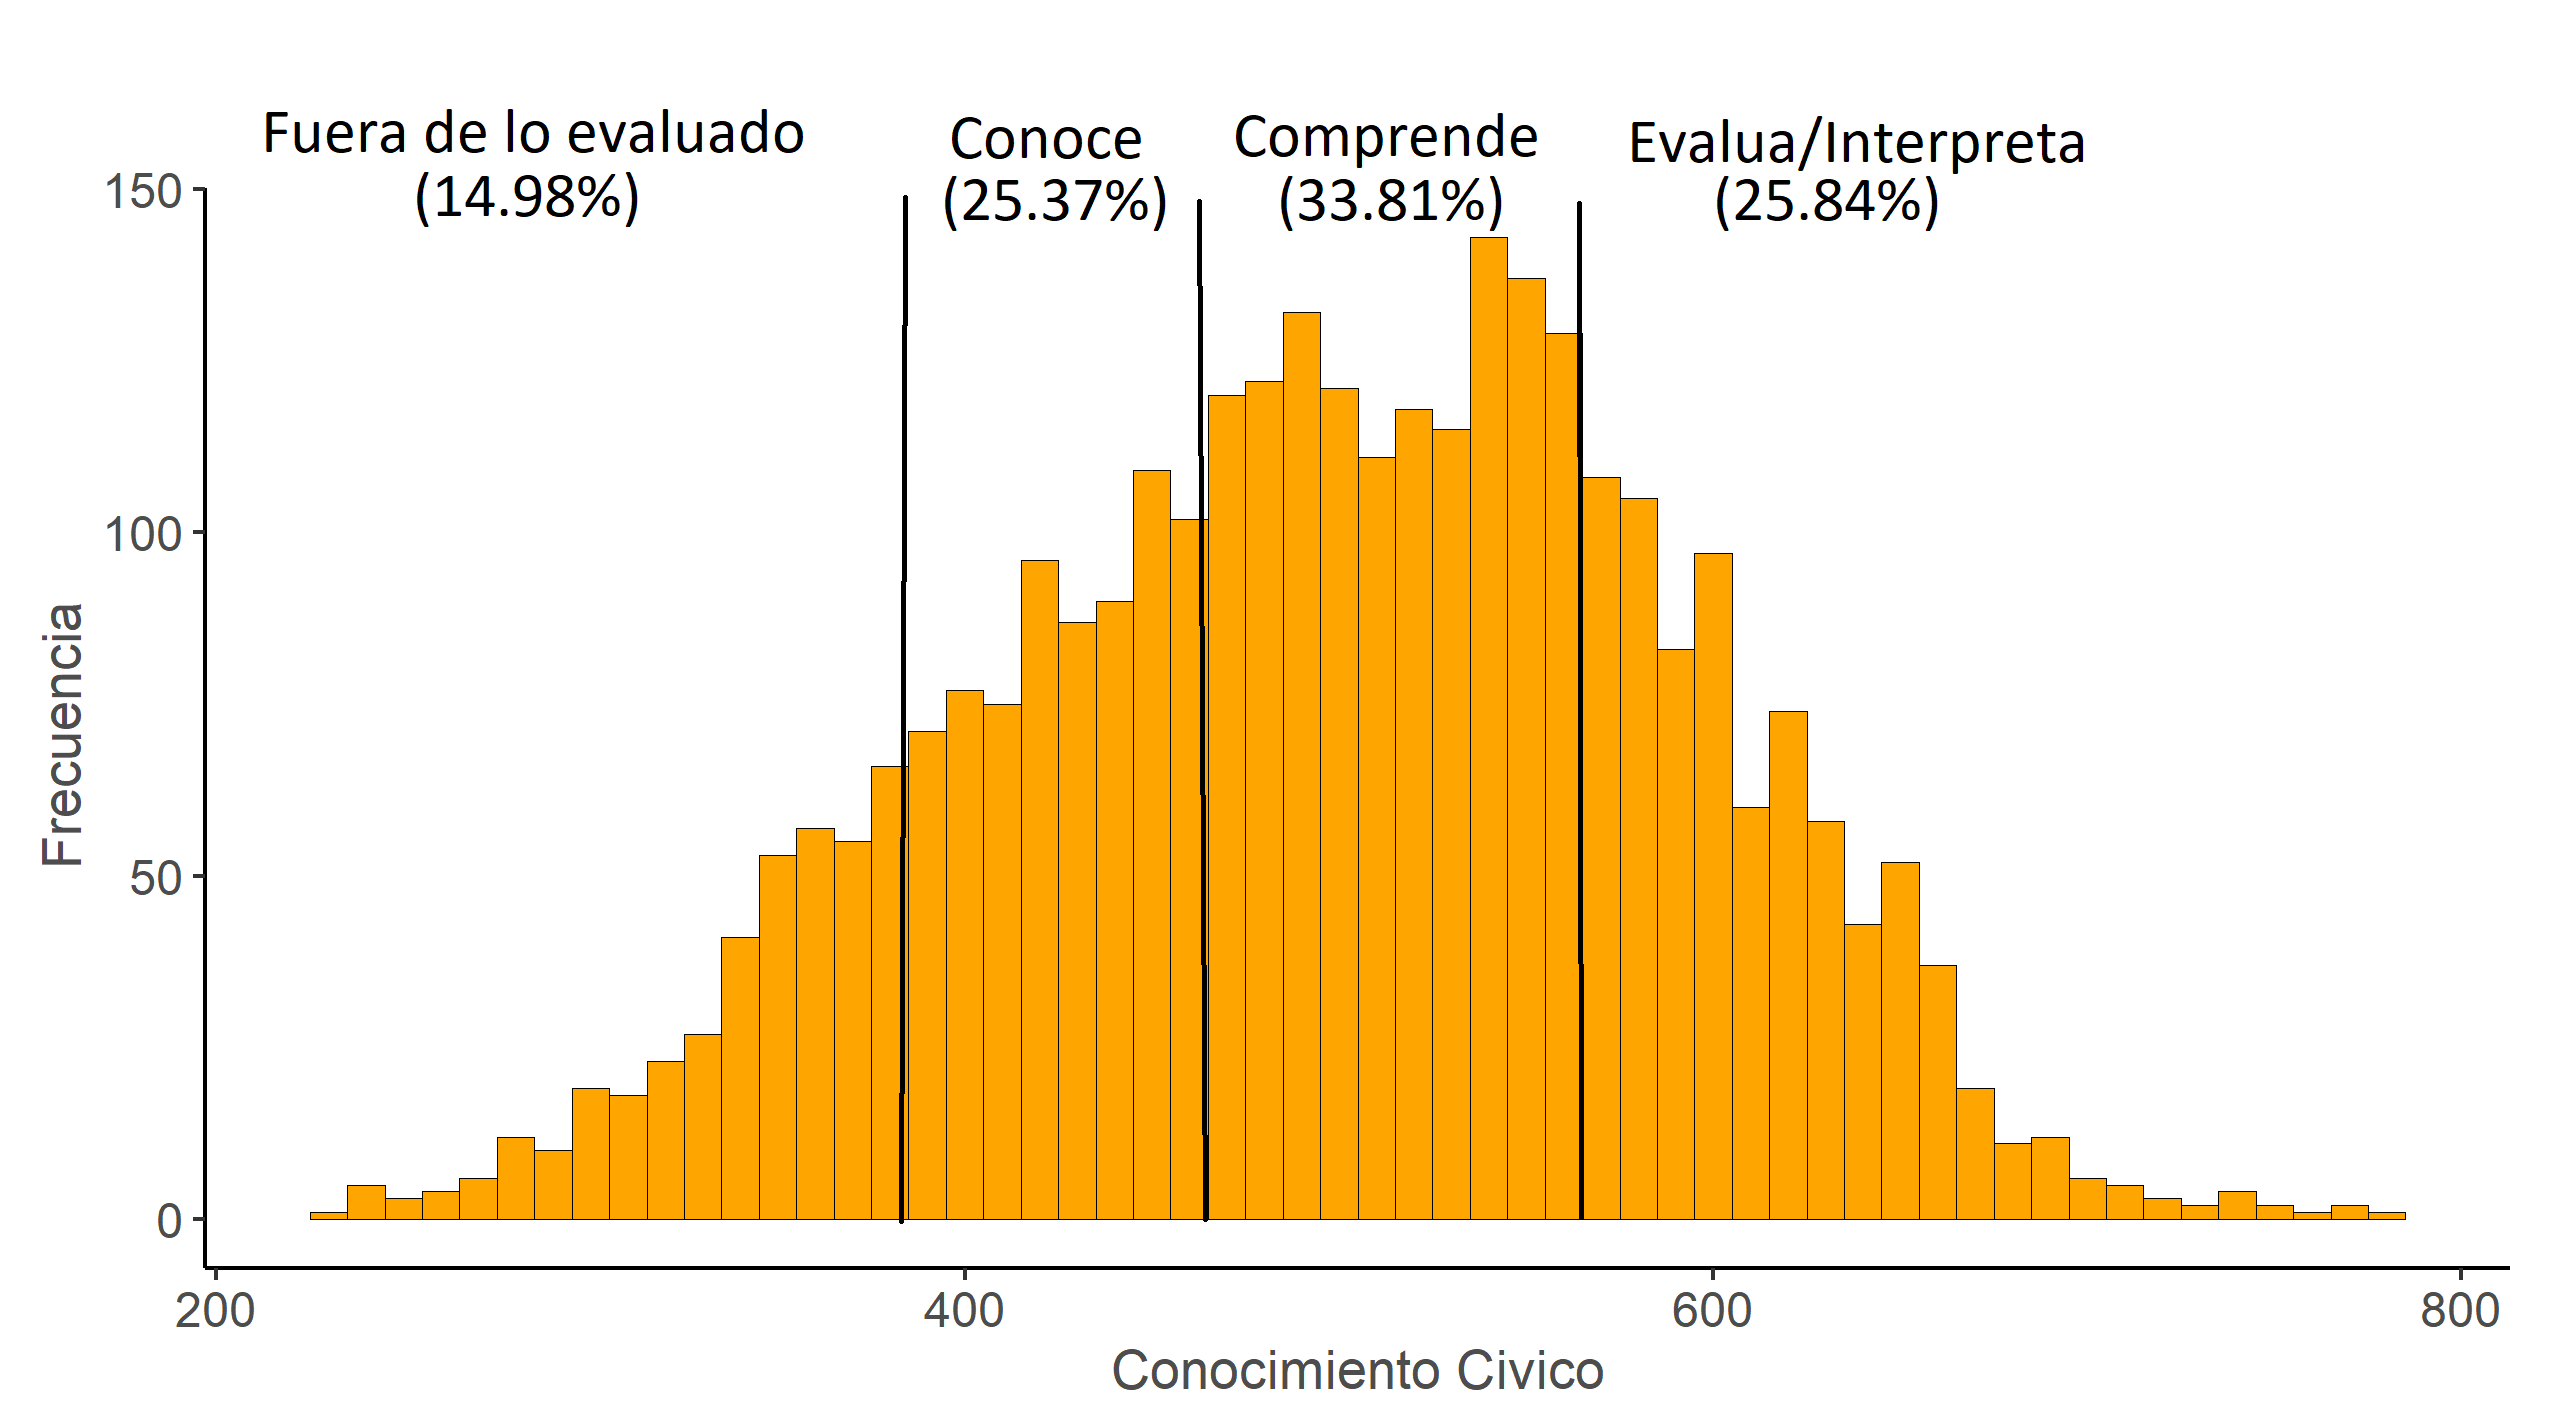
\includegraphics[width=1.1\linewidth,]{images/dist} 

}

\caption{Distribición del Conocimiento Civico}\label{fig:unnamed-chunk-7}
\end{figure}

\newpage

El grafico posterior corresponde a la distribución de la comprensión lectora, prueba en la cual se muestra un peor desempeño que en la prueba de conocimiento cívico. Dos de cada cinco estudiantes poseen una comprensión lectora insuficiente, mientras que menos de uno cada cuatro posee un nivel adecuado.

Esto da cuenta de un problema muy preocupante, ya que implica que buena parte de los estudiantes no poseen un desarrollo adecuado de habilidades como la comprensión, la interpretación o el análisis, habilidades las cuales hemos argumentado son fundamentales para la vida ciudadana.

\begin{figure}[!ht]

{\centering 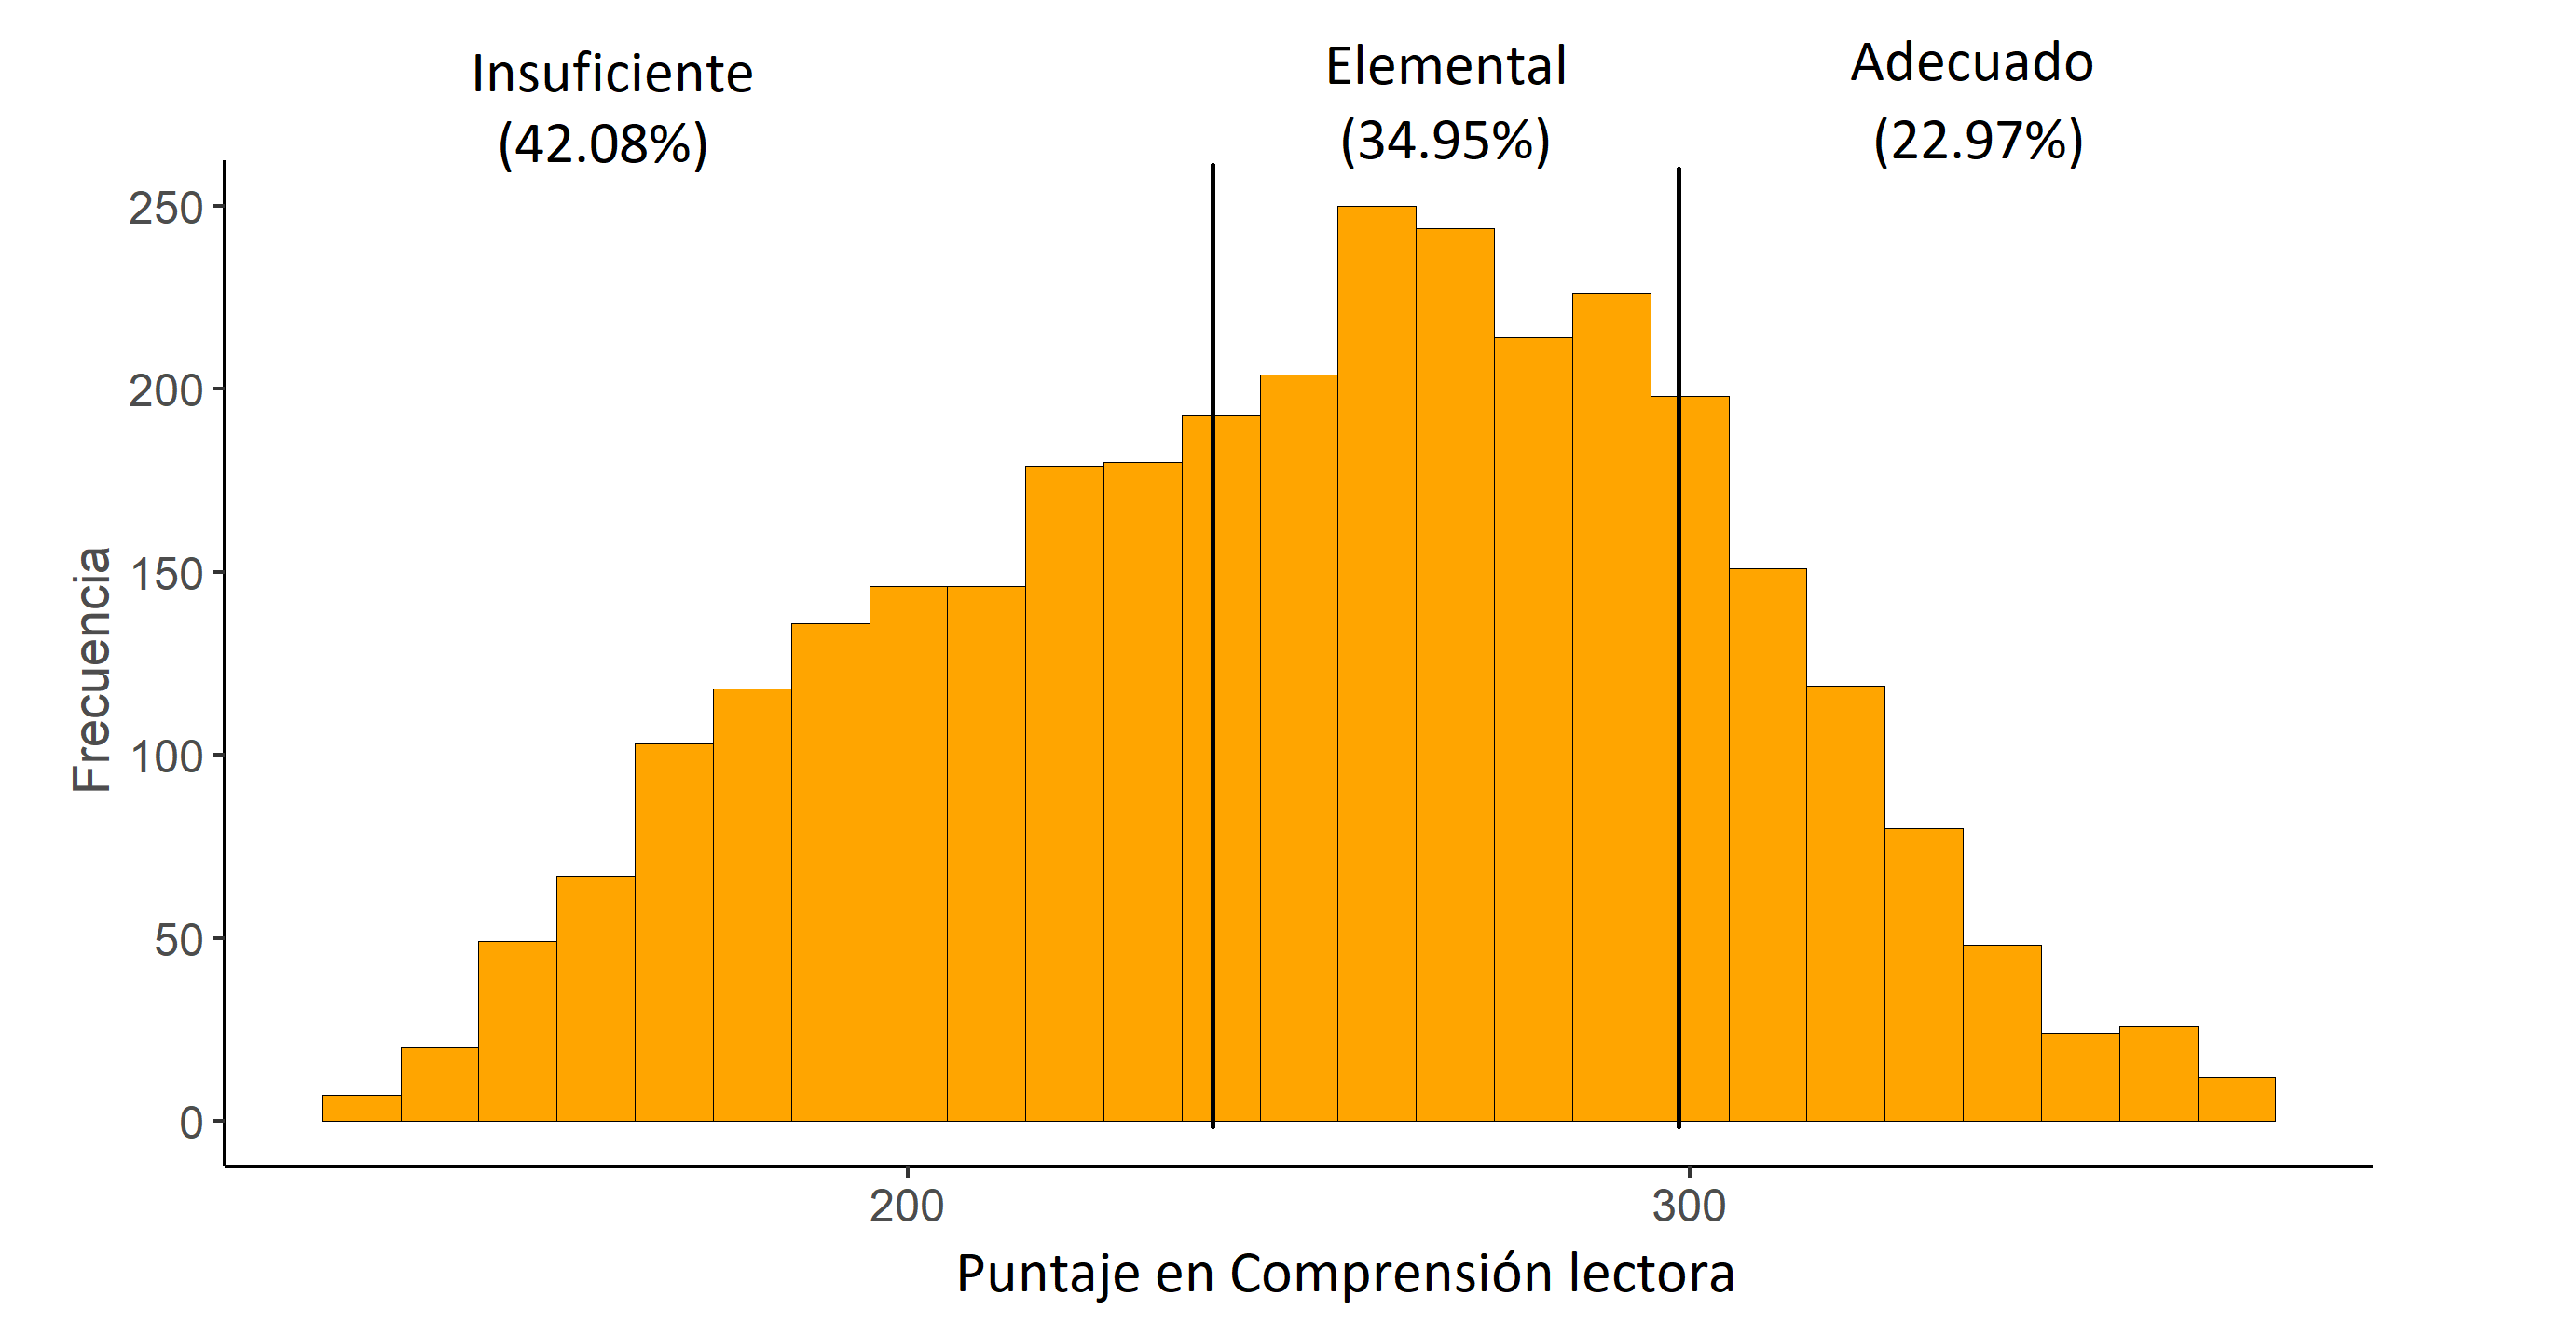
\includegraphics[width=1.1\linewidth,]{images/dist2} 

}

\caption{Distribición de la Comprensión lectora}\label{fig:unnamed-chunk-8}
\end{figure}

\newpage

\hypertarget{anuxe1lisis-relaciuxf3nal}{%
\section{Análisis relaciónal}\label{anuxe1lisis-relaciuxf3nal}}

Retomando nuestra hipótesis y robusteciéndola con las definiciones planteadas, podemos decir que el manejo del lenguaje, como herramienta del razonamiento, posee una influencia positiva en las habilidades políticas necesarias para la vida ciudadana, entre las cuales destacan la comprensión, la interpretación y la evaluación. Igualmente podemos decir que ambos conceptos son bien medidos por la prueba de conocimiento cívico y ciudadano, así como por las pruebas de lectura. Antes de entrar en el trabajo de datos de esta investigación (que será con las bases ICCS y SIMCE), se presenta una evidencia preliminar. A continuación, se puede observar un gráfico que expone la relación a nivel internacional, entre los promedios de los estudiantes por país de las pruebas de comprensión lectora de la prueba pisa y el conocimiento cívico de la ICCS.

\begin{figure}[!ht]

{\centering 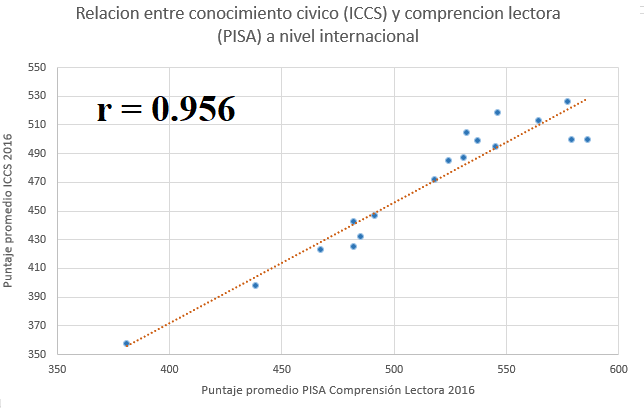
\includegraphics[width=1\linewidth,]{images/relacionmacro} 

}

\caption{relación internaciónal}\label{fig:unnamed-chunk-9}
\end{figure}

Como puede apreciarse, a nivel internacional, existe una estrecha relación entre ambas variables. Según esta relación, países con mayores niveles de comprensión lectora poseen igualmente mayores niveles de conocimiento cívico y ciudadano. Como se expone en la imagen, existe una relación de alta intensidad entre ambas variables (r = .95). No obstante, no hay que dejarse engañar por esta relación por dos razones. En primer lugar, esta relación no está controlada por ninguna variable. En segundo lugar, esta relación a nivel países, no nos permite afirmar que exista una relación entre comprensión lectora y conocimiento cívico a nivel individual o a nivel escuela. A continuación presentamos la relación entre el conocimiento civico y la comprension lectora en base a los datos individuales de la base ICCS-SIMCE.

\begin{figure}[!ht]

{\centering 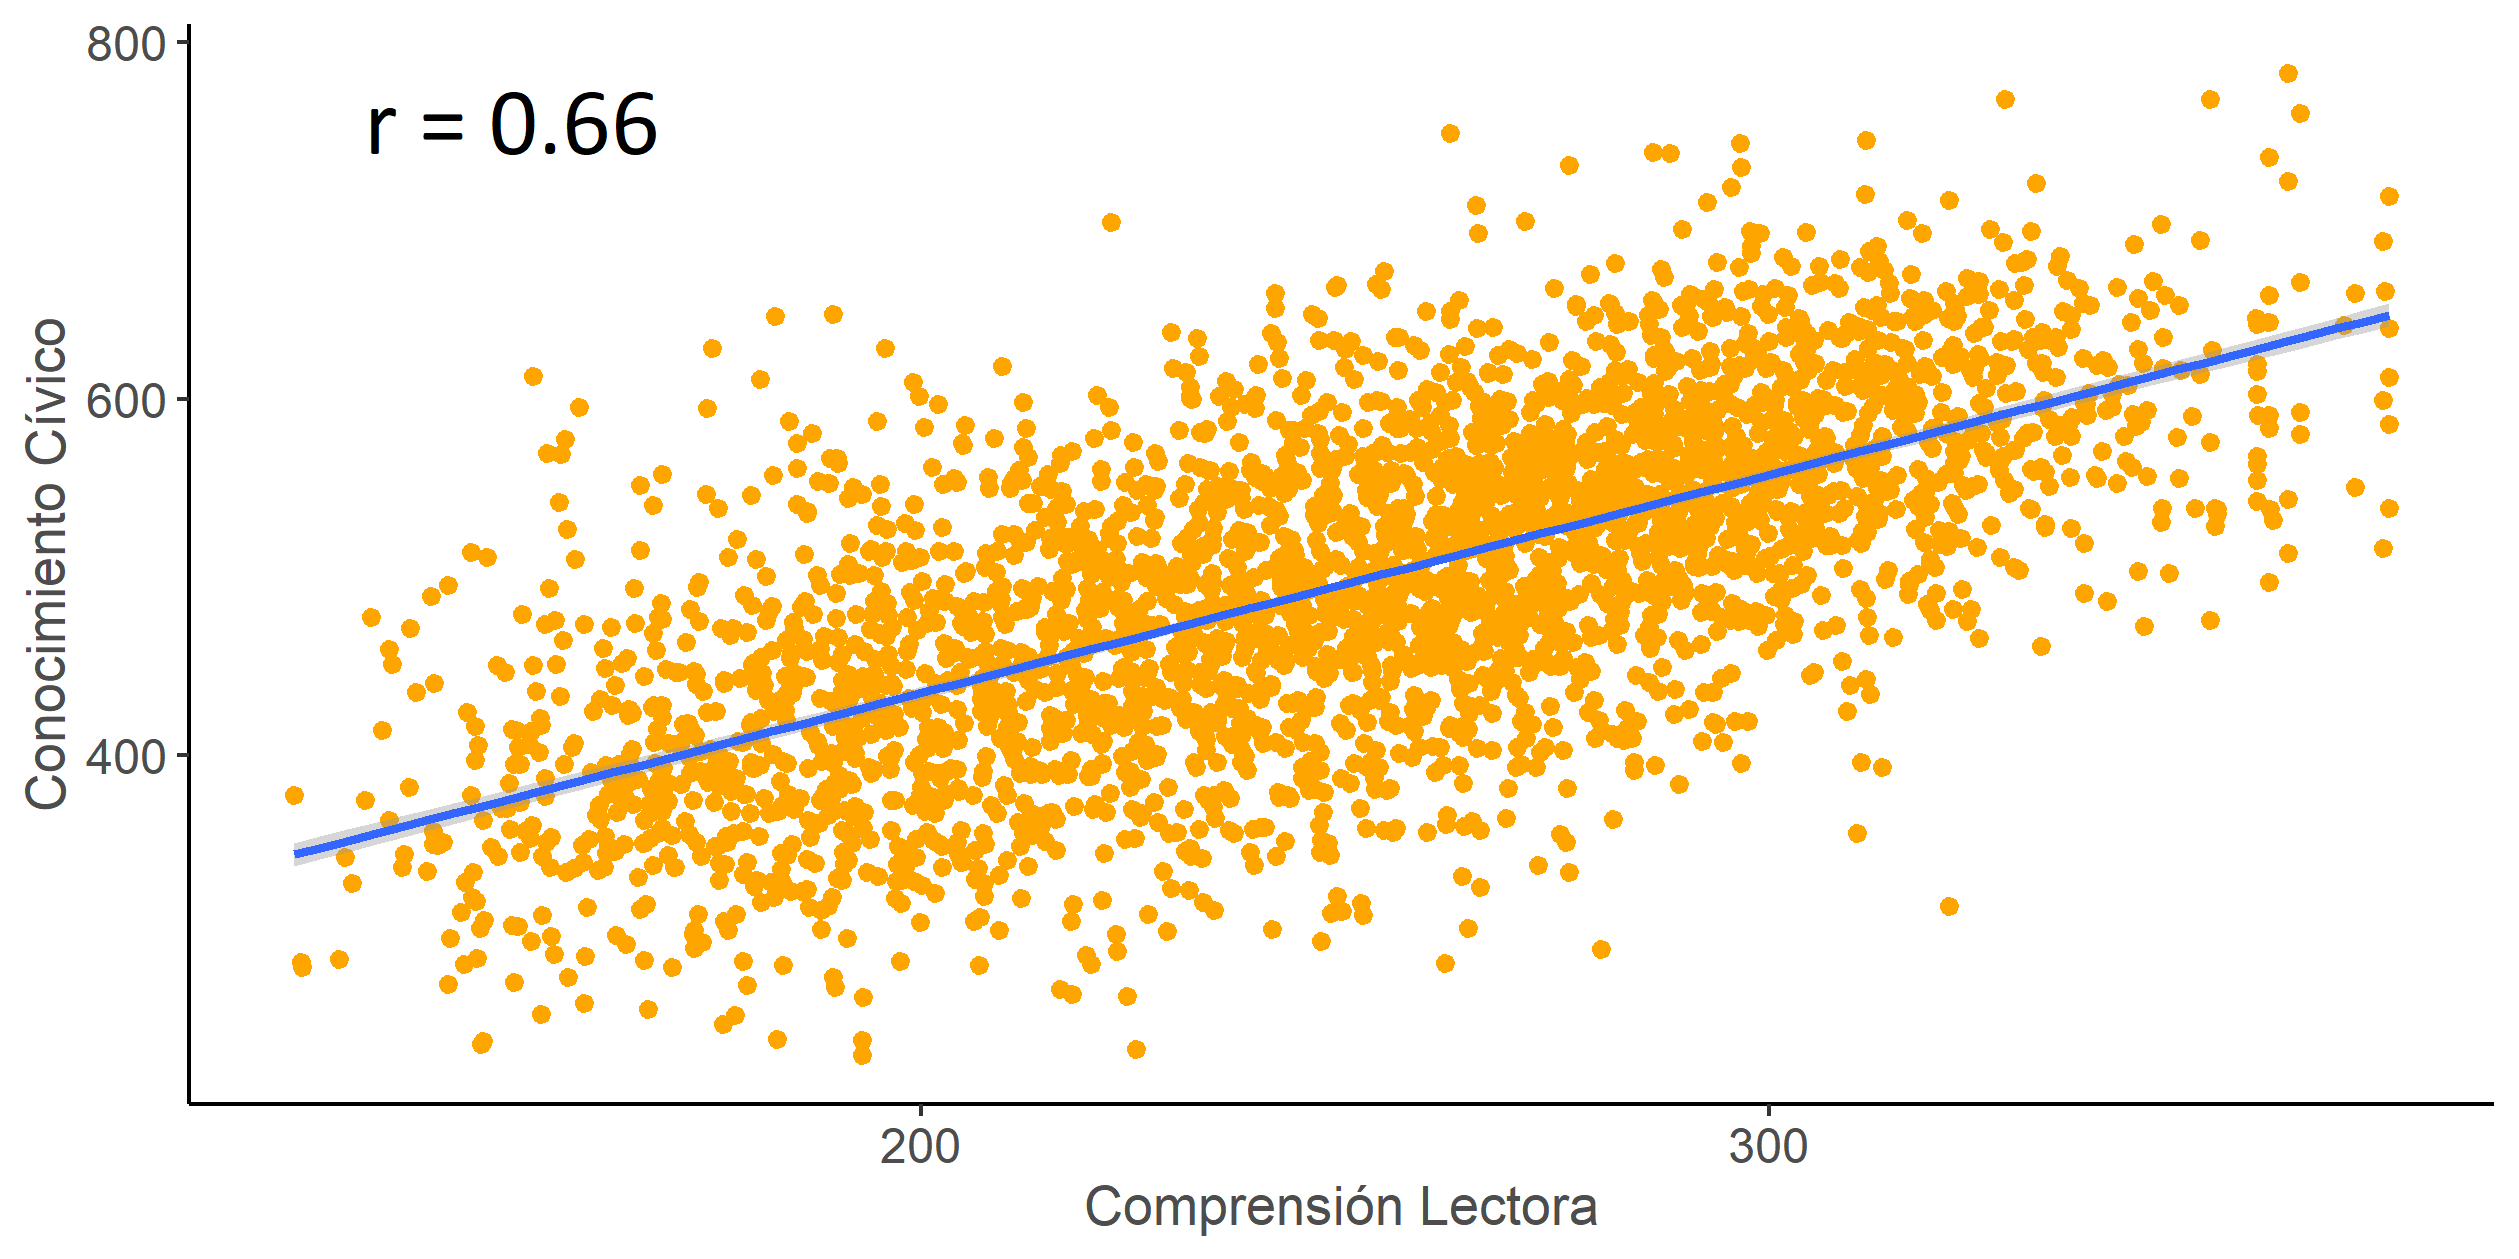
\includegraphics[width=0.8\linewidth,]{images/scater} 

}

\caption{Grafico de nuve}\label{fig:unnamed-chunk-10}
\end{figure}

Como puede verse la relación es igualmente positiva aunque, en relación a lo internacional, disminuye la intensidad De todos modos, se puede apreciar en base a la correlación de pearson una relación de alta intensidad según los parámetros de Cohen (\(r= .66\)).

\begin{verbatim}
## `summarise()` has grouped output by 'pleng_rang'. You can override using the `.groups` argument.
\end{verbatim}

\begin{figure}[!ht]

{\centering 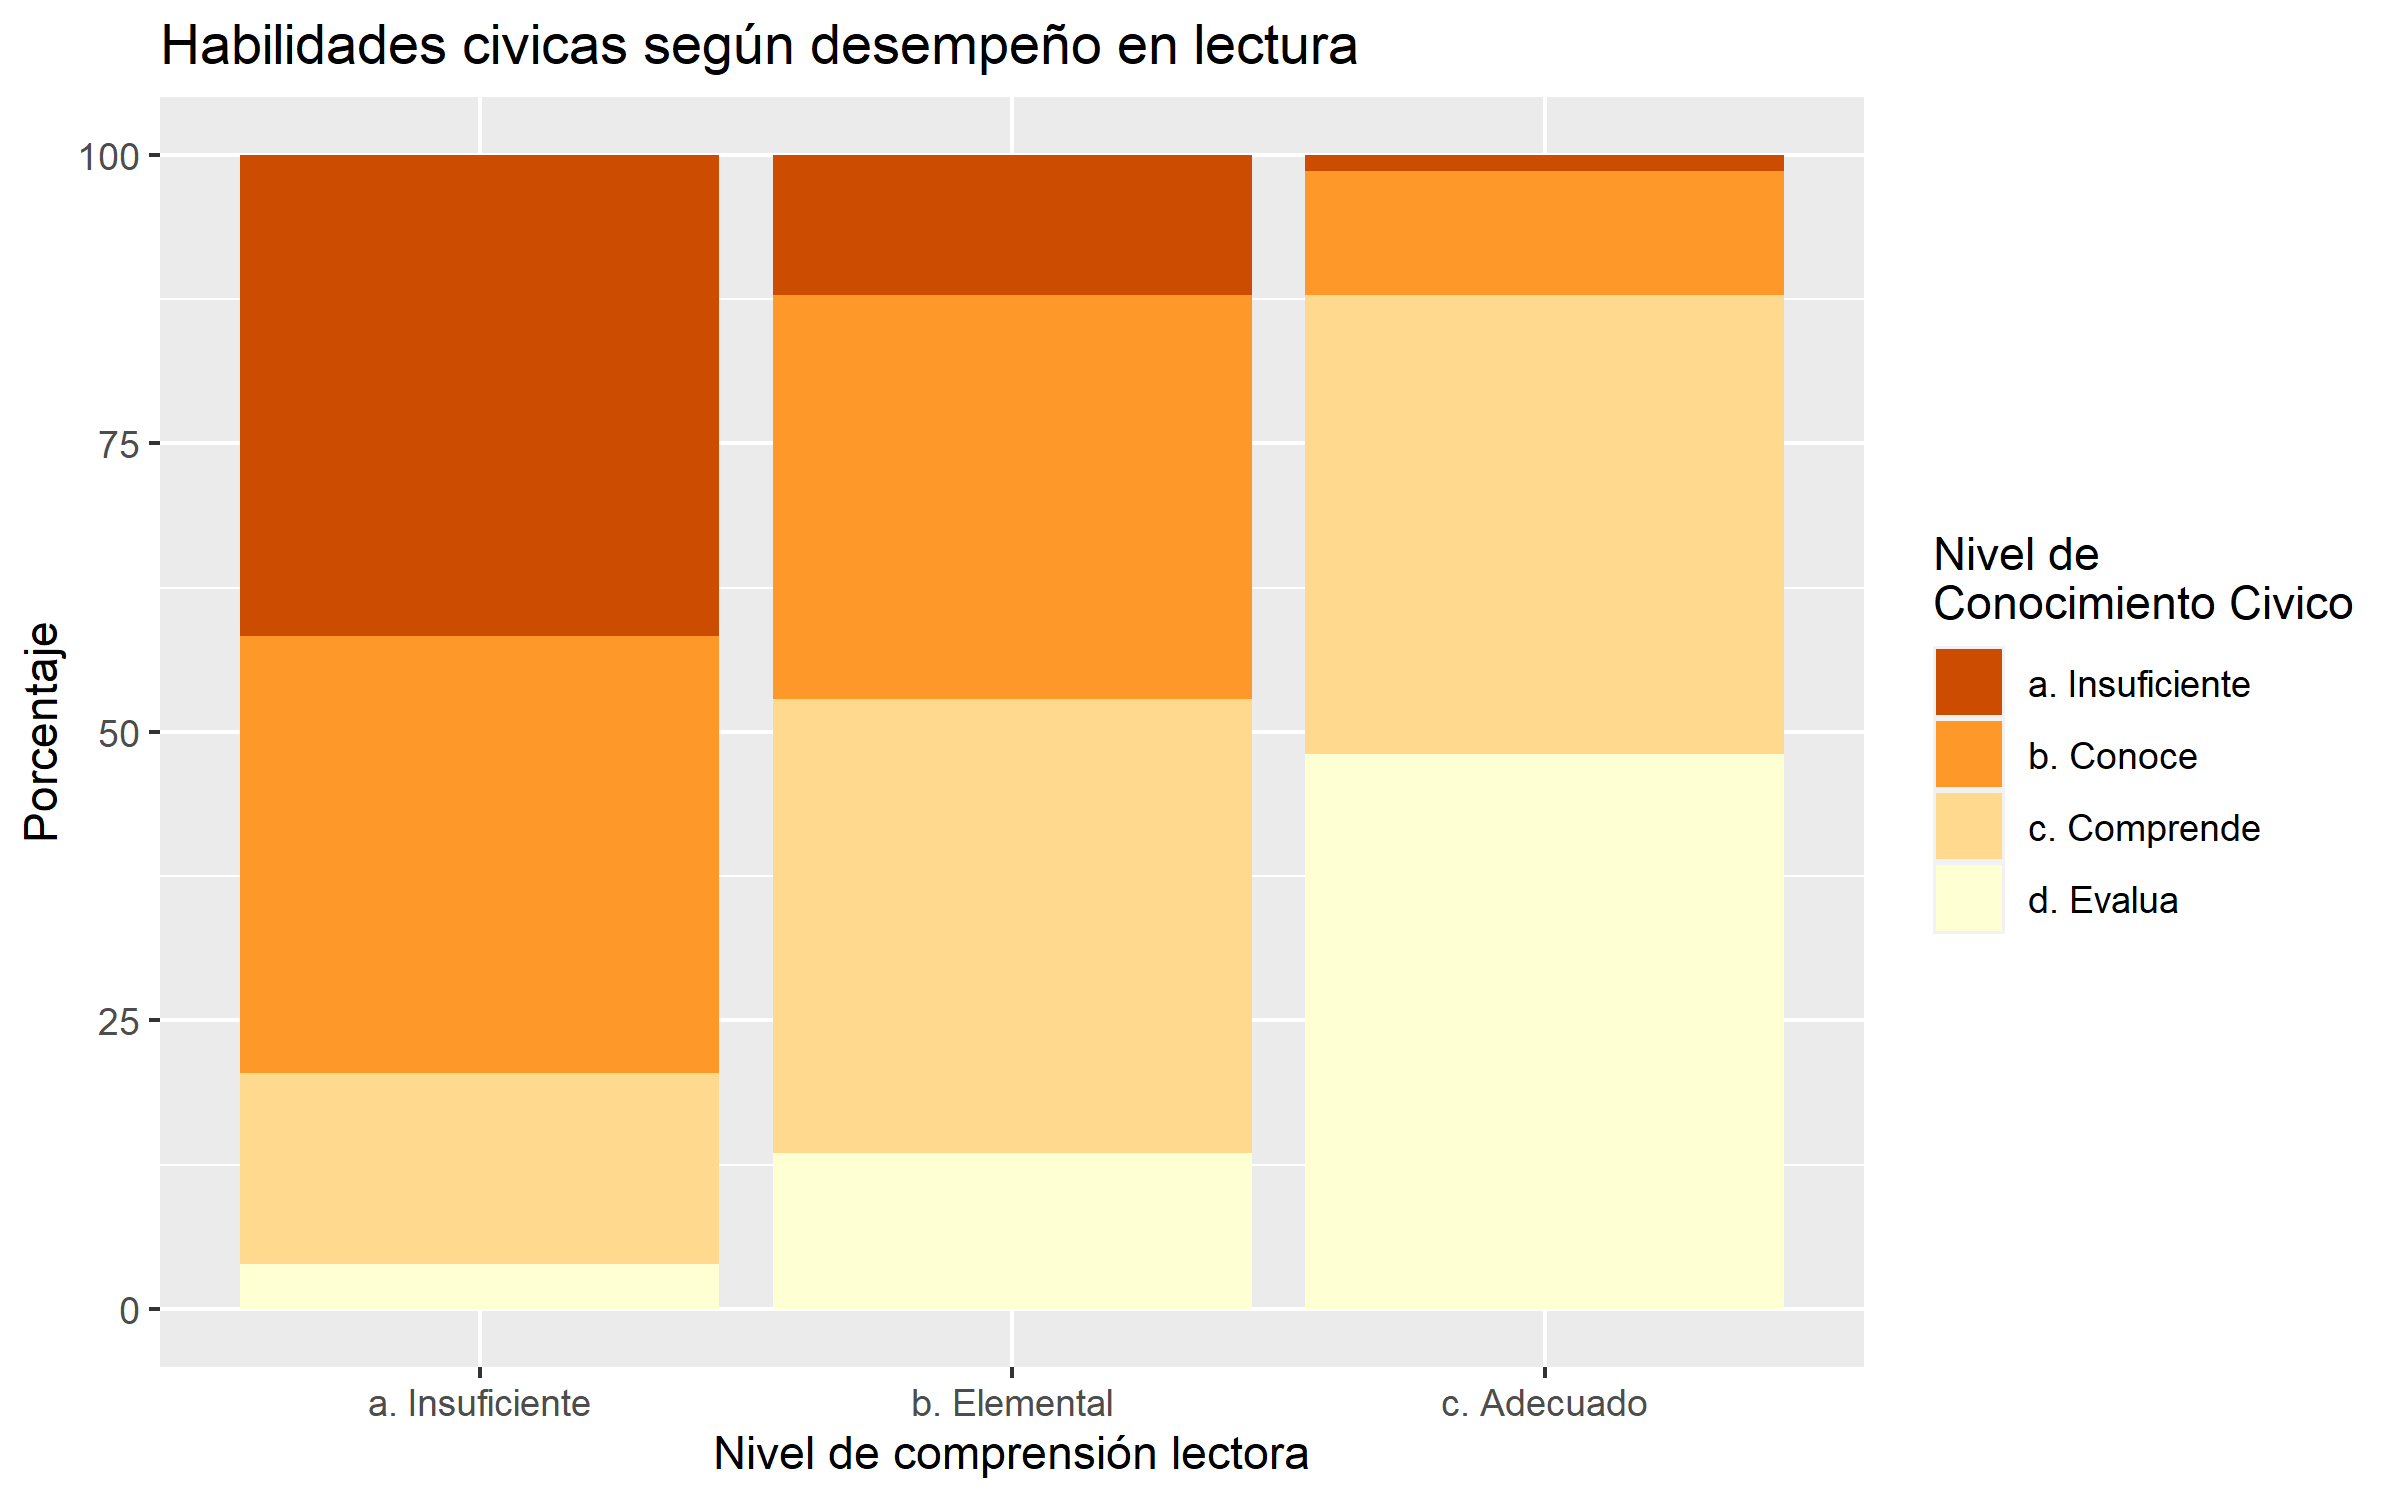
\includegraphics[width=0.8\linewidth,]{images/graficobivariadocategorico} 

}

\caption{Niveles de conocimiento civico según comprensión lectora}\label{fig:unnamed-chunk-12}
\end{figure}

El grafico de la figura numero 9.5, resulta sumamente ilustrativo del punto que busca señalar esta tesis. Para entender el grafico debemos comprender que se esta graficando la relación entre los niveles de conocimiento cívico y los niveles de manejo del lenguaje. Los niveles de manejo del lenguaje se clasifican en insuficiente, elemental y adecuado, mientras que los niveles de conocimiento cívico no refieren a que tan aceptable son los resultados, sino hasta que habilidad logran desarrollar los estudiantes en la prueba de formación ciudadana. Como se mencionó anteriormente para responder bien la prueba de cívica no solo es necesario poseer un amplio conocimiento de memoria sobre asuntos cívicos y ciudadanos. Más bien es necesario tener habilidades para poder interpretar situaciones políticas. Al respecto la habilidad más compleja es la de evaluar, la cual puede comprenderse según los evaluadores como dar cuenta de la postura de un enunciado o evaluar críticamente su pertinencia en determinada situación. Analicemos minuciosamente la distribución de cada uno de los conjuntos de barras.

El primer conjunto de barras refiere a las personas que son calificadas como insuficientes en la prueba de conocimiento cívico. Esta clasificación es bastante deprimente, pues implica que esos estudiantes no poseen el nivel mínimo que busca medir la prueba. Por decirlo asi, quedan por debajo de la regla de medición. Como vimos anteriormente aproximadamente el 15\% de los estudiantes se encuentra en esta categoría. Entre ellos, es notorio, observando los colores que prácticamente se trata de estudiantes con niveles deficientes de manejo del lenguaje. Casi todos los que pertenecen a este grupo comparten la característica de poseen una mala calificación en la prueba de comprensión lectora. Esto va en línea con nuestra hipótesis.

El segundo grupo corresponde a quienes logran demostrar sus conocimientos en la prueba, pero no sus habilidades. En este grupo siguen siendo preminentes los estudiantes que poseen un nivel menor al elemental en comprensión lectora. Además, se puede observar que existe una mayor proporción de estudiantes que poseen simplemente un nivel elemental de lectura pero que no es adecuado para su grado de estudio.

En el tercer grupo se encuentran quienes demostraron poseer la capacidad de comprender situaciones políticas. Esta es una habilidad fundamental para el mundo político, pues comprenderlo es parte esencial del proceso para participar de él. En este grupo, la mayoría de los estudiantes poseen un nivel de lectura elemental, pero no adecuado para su nivel. Seguidamente, el grupo que más destaca después del elemental es quienes poseen un nivel insuficiente manejo del lenguaje. Finalmente, en este grupo a diferencia de los dos anteriores es más considerable la proporción de estudiantes que poseen un nivel adecuado, mas no sobresaliente. Quizás seria bueno para versiones posteriores incluir la categoría sobresaliente en lenguaje.

El ultimo grupo corresponde a quienes poseen la habilidad de interpretar y evaluar situaciones políticas. Esta es una habilidad de alta exigencia cognitiva y requiere el manejo de las habilidades anteriores. Una persona que es capas de interpretar y evaluar propuestas políticas esta mucho más preparada para la ciudadanía, especialmente desde una perspectiva del actor crítico, pues tendrá herramientas para esa crítica. Es este en el único grupo que se encuentra una prevalencia de las personas con una lectura adecuada y el único grupo donde la presencia de estudiantes con una lectura deficiente es casi marginal. De todos modos, resulta interesante profundizar en aquellos casos que logran poseen habilidades de evaluación sin un buen manejo del lenguaje.

Lo evidenciado en esta descripción de los datos va en dirección de lo planteado en las hipótesis. Mientras mejores son las habilidades lingüísticas del estudiante, más probable parece ser que este posea buenas habilidades para la vida cívica y ciudadana. Para comprobar estos resultados preliminares recurriremos las regresiones multinivel que responden mejor a las condiciones de los datos a analizar.

\hypertarget{modelos}{%
\section{Modelos}\label{modelos}}

\hypertarget{analisis-multinivel-varianza-entre-escuelas}{%
\subsection{Analisis Multinivel: Varianza entre escuelas}\label{analisis-multinivel-varianza-entre-escuelas}}

A partir del modelo nulo, utilizando la varianza entre grupos y residual, se calculo la correlación intraclase, es decir, la proporción de la varianza del conocimiento civico que es explicada por el nivel escuela. Prácticamente un tercio de la varianza del conocimiento civico depende del nivel escolar y agregado, lo que da cuenta de la importancia de controlar por estas variables asi como de investigar que cualidades de la escuela fomentan el conocimiento cívico.

\begin{figure}[!ht]

{\centering 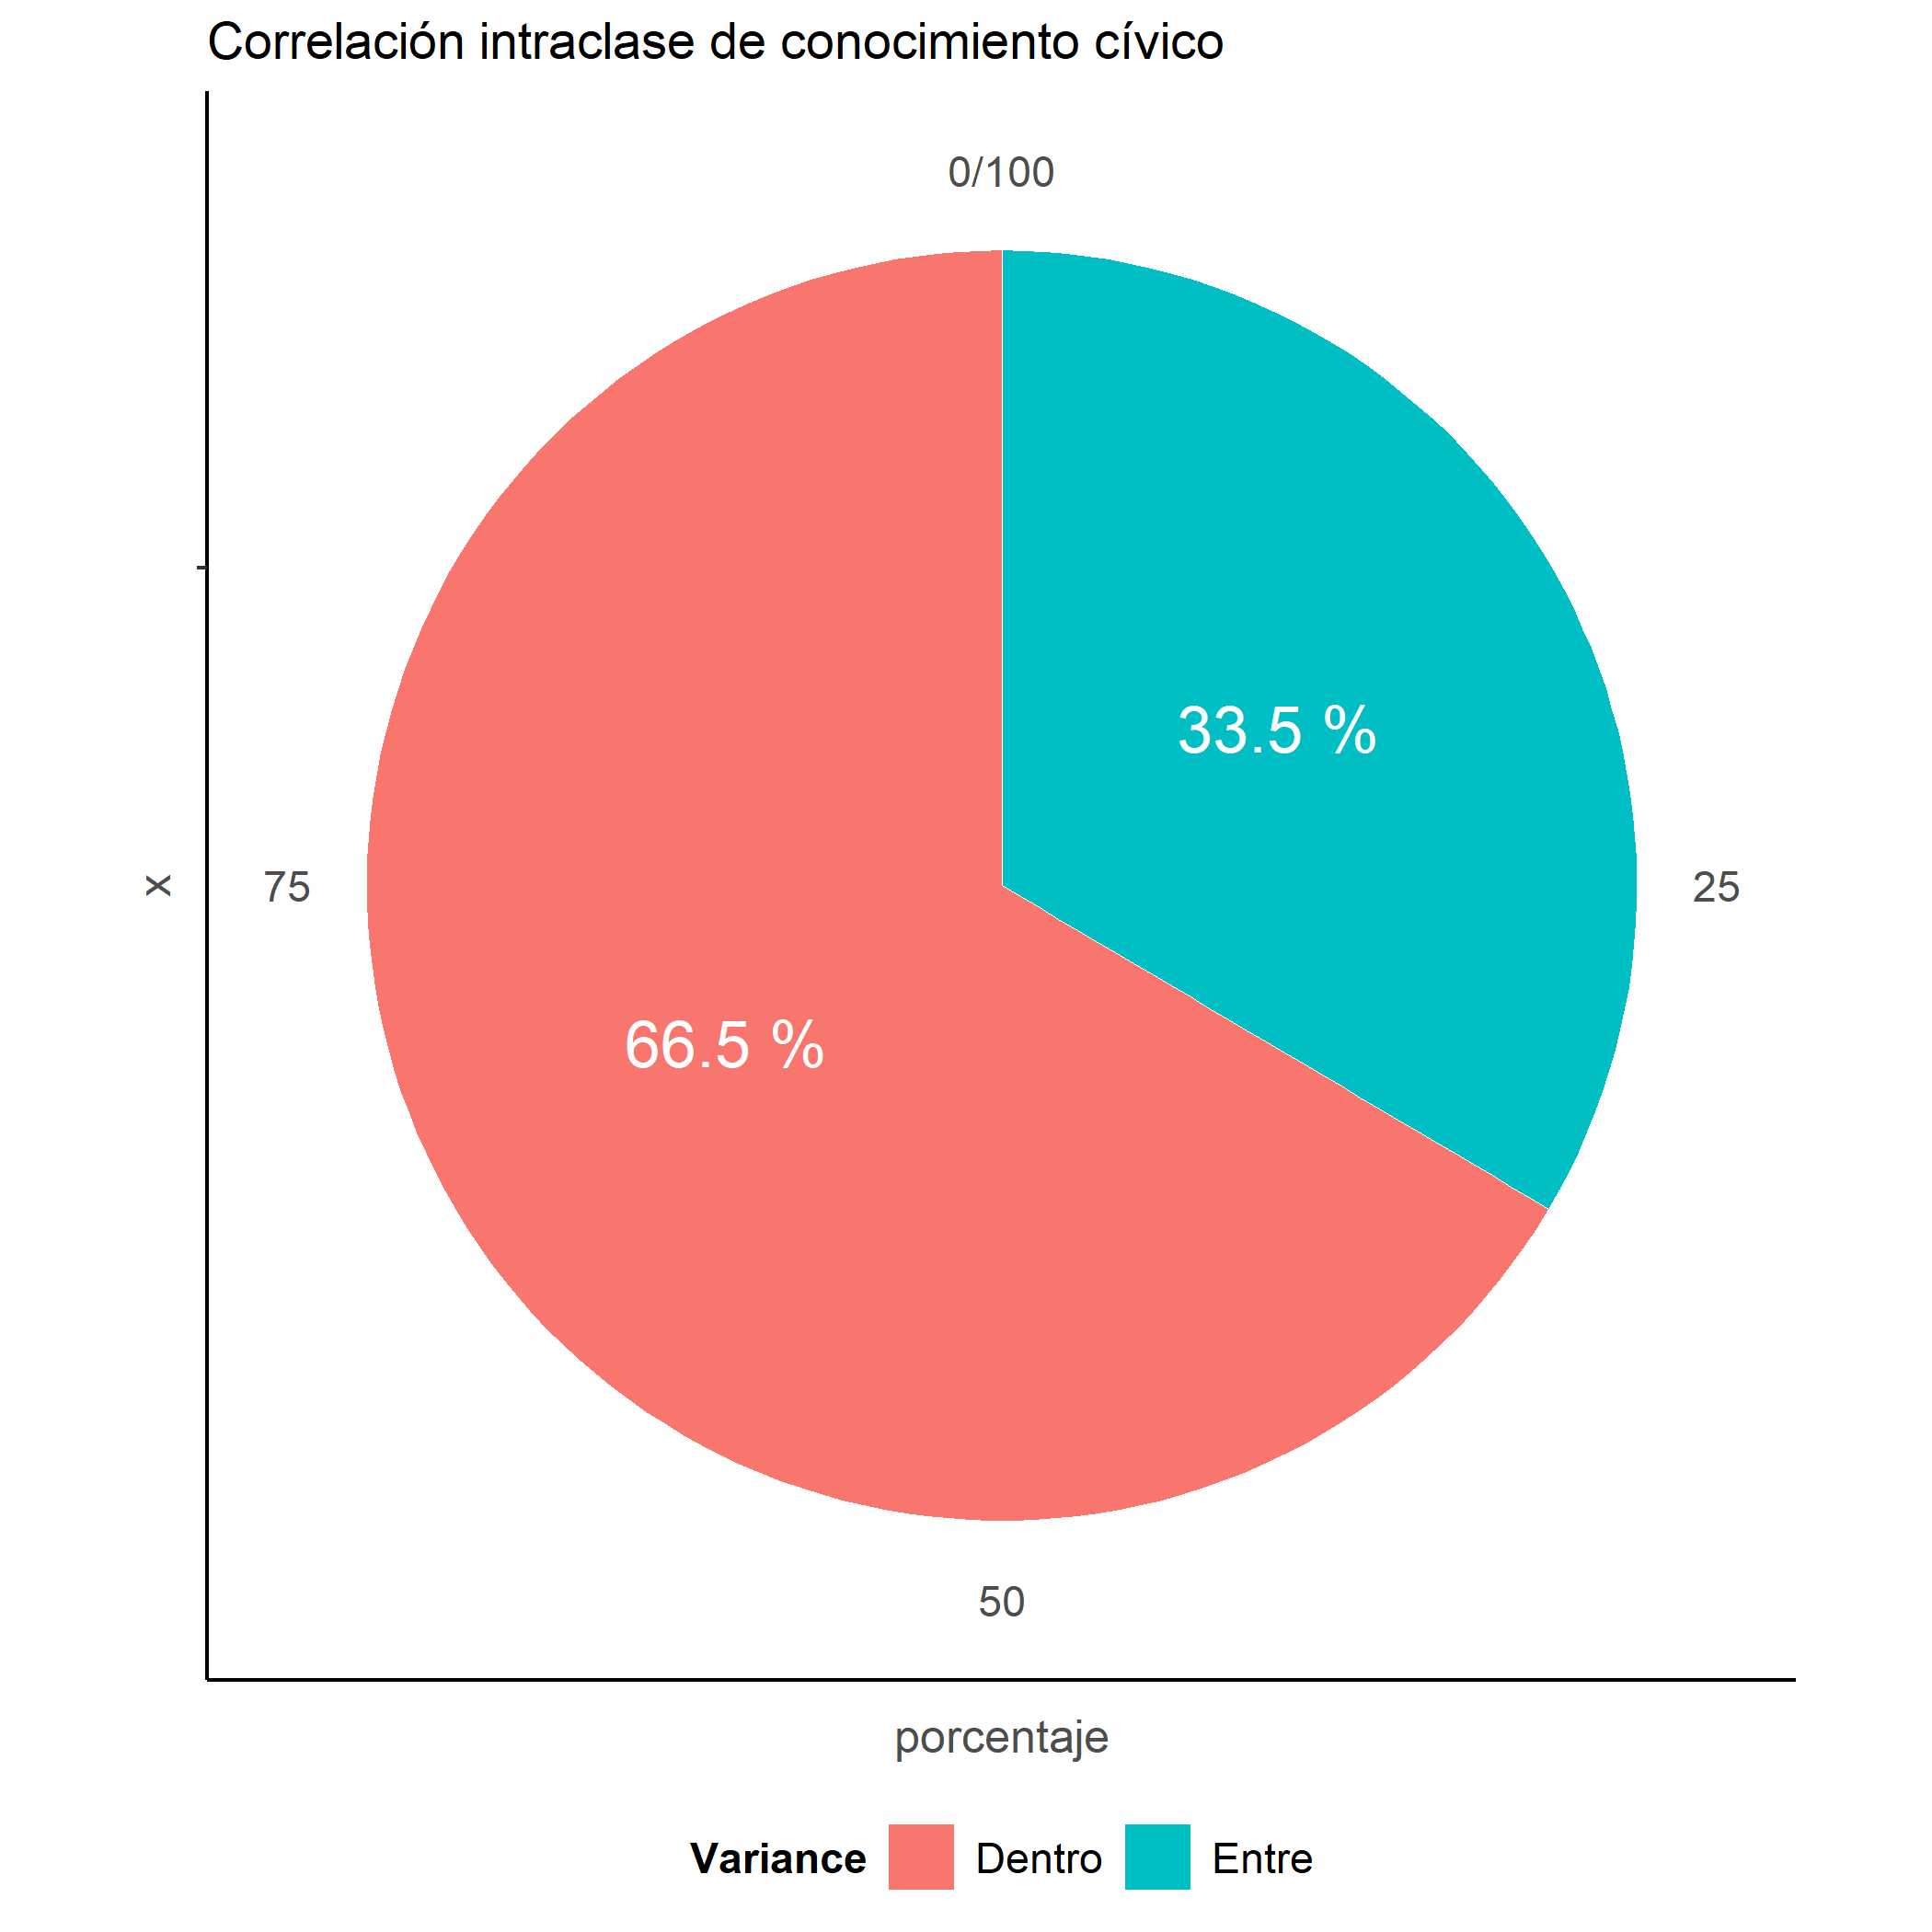
\includegraphics[width=0.5\linewidth,]{images/iccplot} 

}

\caption{Proporción de varianza entre y dentro}\label{fig:unnamed-chunk-13}
\end{figure}

\newpage

\hypertarget{resultados-del-anuxe1lisis-multinivel-efectos-e-interacciuxf3n.}{%
\subsection{Resultados del análisis multinivel: efectos e interacción.}\label{resultados-del-anuxe1lisis-multinivel-efectos-e-interacciuxf3n.}}

En la tabla consecutiva se presentan 4 modelos multinivel los cuales son todos significativamente mejores que el anterior. El primer modelo incluye las variables de reproducción social, el segundo, incluye una variable de la escuela, el tercero agrega el interés político social del estudiante. El cuarto incluye la variable puntaje en la prueba Simce de lenguaje, y el quinto expone la aleatorización de la pendiente y la interacción de una variable nivel dos: el promedio del nivel socioeconómico.

\begin{center}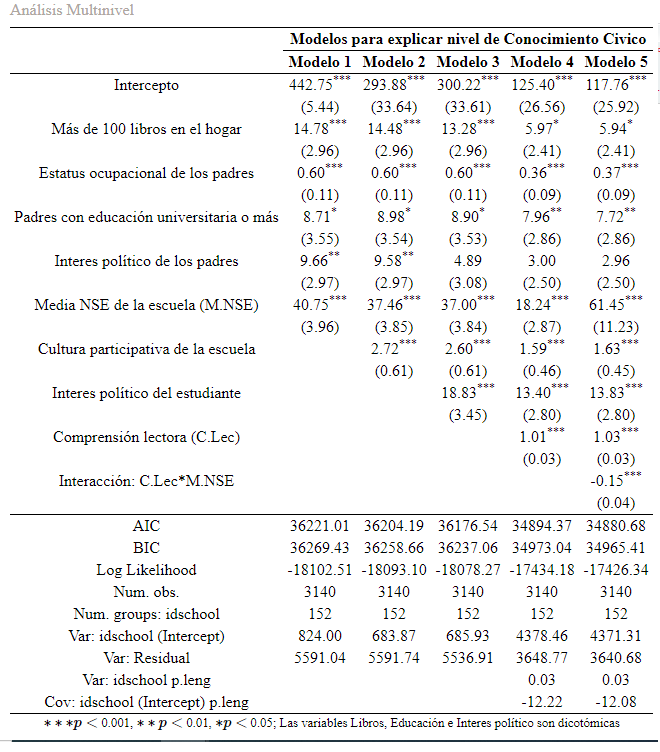
\includegraphics[width=1.2\linewidth,]{images/regmultinivel} \end{center}

El primer modelo incluye aquellas variables que representan la reproducción social de la desigualdad política, y como puede verse, todas estas variables poseen un efecto significativo que implica cambios de puntajes que van aproximadamente desde 10 a 40 puntos. Así, poseer más de 100 libros en la casa, aumenta 14 puntos el conocimiento cívico, por su parte la variable ocupación posee un efecto considerable, en un rango de más de 80 valores, por cada unidad que aumenta el índice de estatus ocupacional el estudiante aumentó 0.6 puntos en la prueba de conocimiento cívico, así por ejemplo poseer 50 pts. más de estatus ocupacional implica aumentar 30 pts. en la prueba de conocimiento cívico. Respecto al efecto de la educación de los padres, este es ambivalente, puesto que si bien es respaldado por la literatura, en vista de los controles aplicados parece solo tener un efecto significativo con un 95\% de confianza, criterio demasiado laxo para una muestra de más de 3000 casos. En último lugar, considerando la variable de segundo nivel, promedio del nivel socioeconómico de los padres del colegio, podemos decir que existe un gran peso del contexto socioeconómico del colegio.

El segundo modelo incorpora una variable del contexto educativo, esta variable da cuenta de que tan de acuerdo están los estudiantes en general con que la participación en la escuela y la comunidad son beneficiosos para la comunidad. Como puede verse, por cada punto que aumenta este promedio mejora en 2 puntos el conocimiento cívico, lo cual reafirma la hipótesis de que un contexto de participación es útil para mejorar el conocimiento cívico de los estudiantes. Cabe destacar que el incorporar esta variable no logra controlar las variables de origen familiar, lo que nos da cuenta que las ventajas sociales del conocimiento cívico no pasan por estar en colegios con mejores climas democráticos.

El tercer modelo incorpora la variable interés político del estudiante. Como plantea la teoría, un estudiante que posee intereses sobre una materia posee una ventaja respecto a la misma, premisa que es comprobada en este caso. El que un estudiante posea interés en la política y los asuntos sociales se asocia con tener 19 puntos más en la prueba de conocimiento cívico. Resulta interesante que el efecto de poseer padres interesados por la política, es completamente controlado por el efecto de que el estudiante tenga interés, lo que nos da cuenta de que el efecto de los padres pasa a través de los hijos. Este control nos permite decir que el efecto del nivel socioeconómico y las ventajas en términos de capital cultural no se explican completa, ni medianamente por qué las personas de mayores recursos tengan más intereses en la política, lo cual nos permite desde ya poner en duda las explicaciones que aluden a que el conocimiento cívico es transmitido como valores e intereses de generación en generación. Siendo más específicos, el efecto que más es controlados es el de tener libros en el hogar. Al parecer, el tener libros en la casa se relaciona con estudiantes interesados en la política, que obtuvieron mejores puntajes en esta prueba.

El cuarto modelo es el modelo fundamental de este trabajo. En este modelo las demás variables son controladas por el efecto de la comprensión lectora medida en la prueba simce de lenguaje. Como puede verse cada punto que aumenta alguien en la prueba simce de lenguaje, aumenta 1 punto en la prueba de conocimiento cívico, lo cual es una relación bastante estrecha considerando los rangos de ambas pruebas (hasta 350 pts). Lo más interesante de incorporar esta variable es lo que ocurre con las demás. Como puede verse el efecto de que existan más de 100 libros en el hogar, prácticamente desaparece, pasando de un efecto de 13 a 6 puntos, y perdiendo la significación al 99\%. Por su parte, respecto a la variable de estatus ocupacional de los padres y al nivel socioeconómico promedio del colegio, es bastante sugerente el hecho de que ambos efectos disminuyen casi a la mitad. En vista de estos controles, podemos decir que el efecto de que los padres posean libros en la casa es realmente producido por la influencia que eso ejerce en la comprensión lectora de los estudiantes. Igualmente, podemos decir que casi la mitad del efecto del nivel socioeconómico de los padres en el conocimiento cívico se debe a la influencia de estas posiciones en el buen manejo del lenguaje.

El quinto modelo es un poco más complejo. Primero incorpora la aleatorización de la pendiente del efecto de la comprensión lectora sobre el conocimiento cívico, permitiendo que esta varíe según contextos. Luego, intentamos explicar dicha variación de la pendiente en función del nivel socioeconómico del colegio, para ver si el efecto del lenguaje sobre el conocimiento cívico difiere en contextos socioeconómicos distintos. Como puede verse en la tabla, el efecto es significativo, y mientras mayor es el nivel socioeconómico menos importante es la comprensión lectora. Para graficar esta interacción, invertimos el sentido de esta. De este modo, se presenta a continuación la capacidad del lenguaje de moderar el efecto de la desigualdad producida por el NSE promedio del colegio.

\begin{figure}[!ht]

{\centering 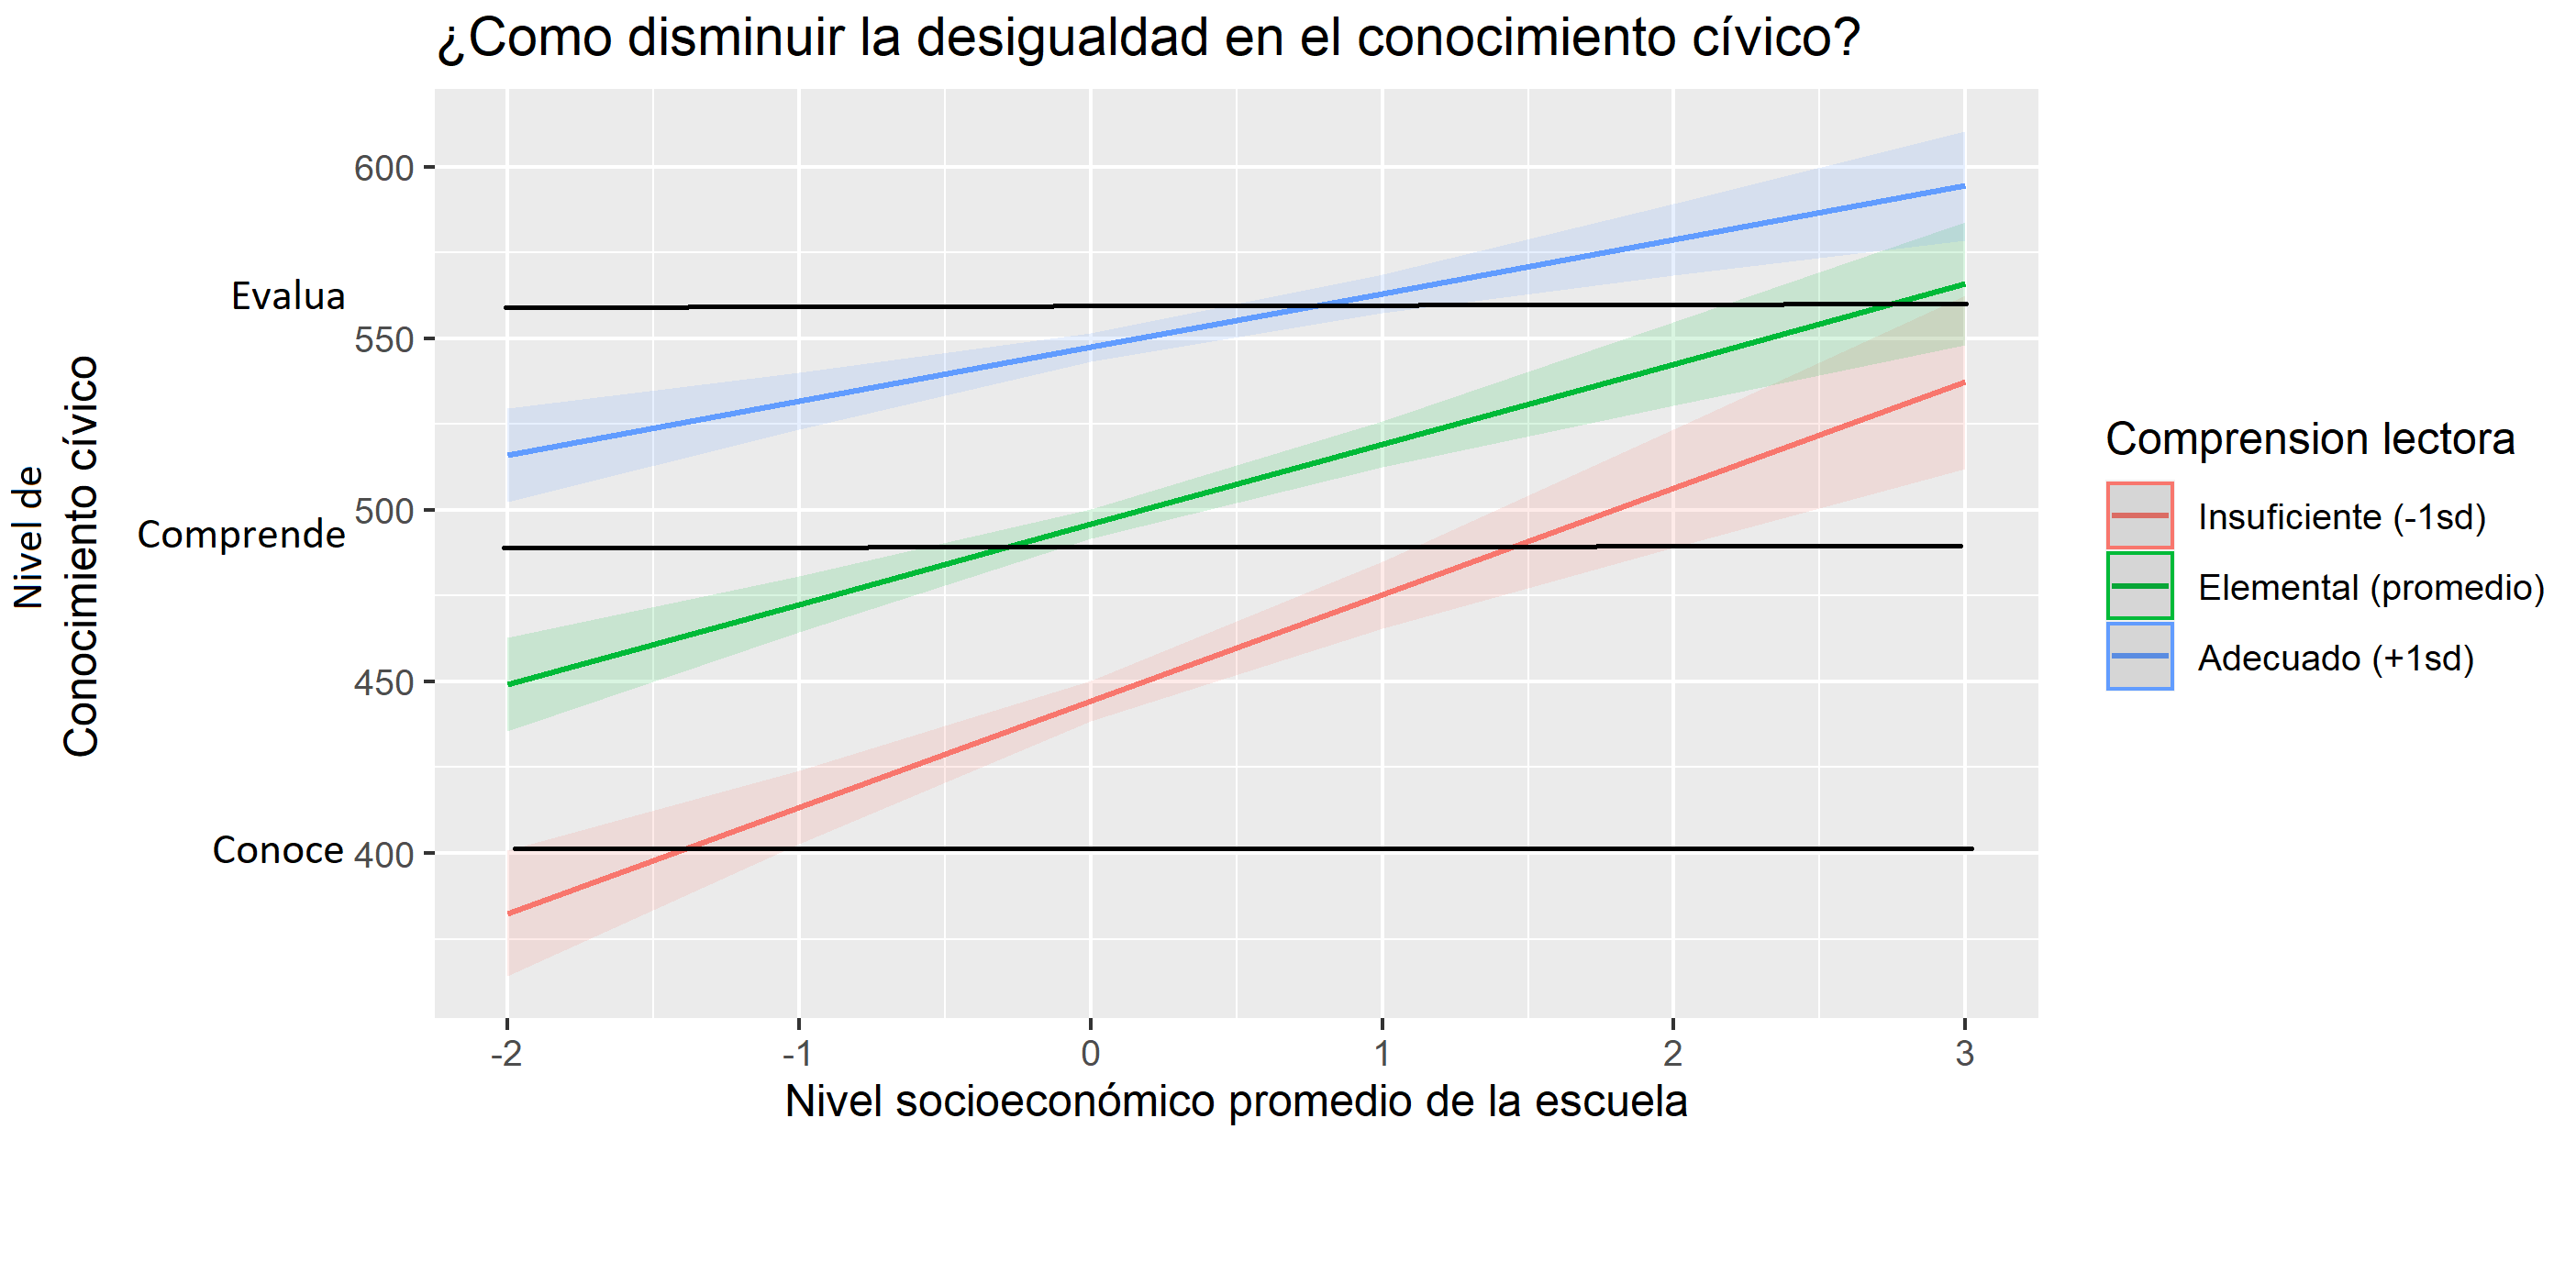
\includegraphics[width=1.2\linewidth,]{images/inter2} 

}

\caption{Interacción}\label{fig:unnamed-chunk-15}
\end{figure}

A partir de esta interacción podemos decir que, aunque la comprensión lectora modera significativamente el efecto del nivel socioeconómico de la escuela, la desigualdad social sigue siendo un problema. Pese a tener una comprensión lectora adecuada, siendo de un colegio de bajos recursos, probablemente un joven no alcance un nivel de habilidad evaluativa en la prueba de conocimiento cívico. Más aun, un joven con adecuado manejo del lenguaje posee el mismo nivel de conocimiento cívico que un joven con manejo lector insuficiente, si es de un colegio de alto estatus. En esta línea, quienes poseen mayores posibilidades de alcanzar un nivel de habilidad Evaluativa en la prueba de la ICCS, son principalmente quienes poseen un manejo adecuado del lenguaje y son de escuelas de alto nse. No obstante, cabe señalar que si se evalúa la pendiente en puntajes muy altos de comprensión lectora los estudiantes de bajos recursos no se encuentran en una gran desventaja frente a sus compañeros de generación más acomodados.

Respecto a la capacidad de este modelo de predecir el conocimiento cívico, se debe señalar que se explica un 75\% de la varianza entre colegios y un 68\% de la varianza individual, lo cual evidencia una alta capacidad predictiva. Respecto al valor total de la varianza el model explica en torno a un 66\% del conocimienoto civico.

\hypertarget{resultados-de-la-mediaciuxf3n-multinivel.}{%
\subsection{Resultados de la mediación multinivel.}\label{resultados-de-la-mediaciuxf3n-multinivel.}}

A continuación, se presentan los resultados del análisis de mediación multinivel. En estos se evalúa la capacidad del lenguaje de explicar la relación entre NSE y conocimiento cívico, haciendo esta evaluación a nivel uno y nivel dos como recomienda la literatura. Para este fin, se evalúa primero, si el NSE se relaciona con lenguaje, luego si el NSE se relaciona con el conocimiento cívico y, posteriormente, si es que el efecto de NSE sobre conocimiento cívico es controlado por la comprensión lectora, repitiendo este proceso en ambos niveles. En la siguiente tabla el nombre de la columna indica la variable dependiente.

\begin{center}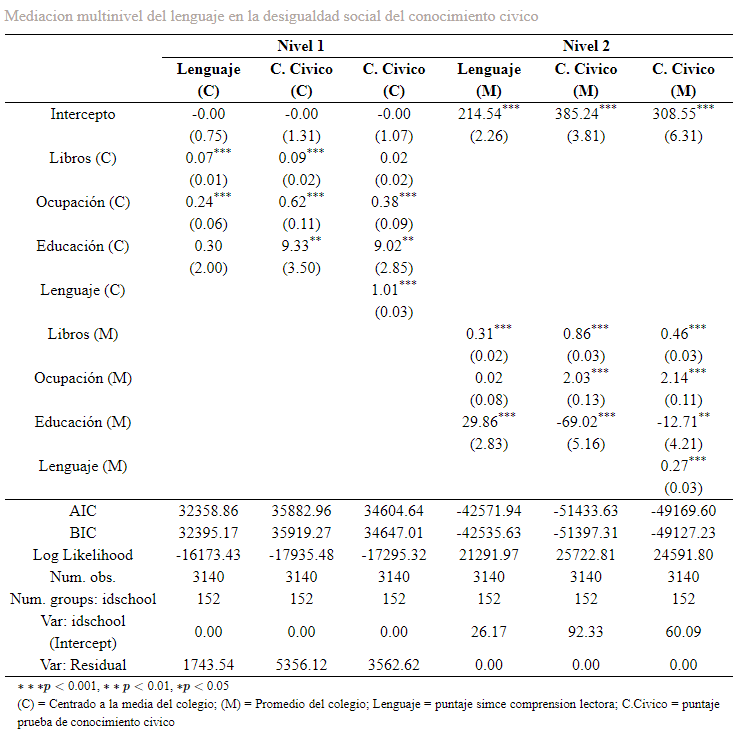
\includegraphics[width=0.8\linewidth,]{images/Mediacion_n1n2} \end{center}

A partir de los resultados de la tabla anterior, es posible concluir que la comprensión lectora posee la capacidad de explicar parcialmente la desigualdad en el conocimiento cívico. En primer lugar en torno al nivel uno, podemos ver que el lenguaje es influido por la cantidad de libros en el hogar y la ocupación de los padres, pero no la educación de los padres. Seguidamente se constata que las tres variables afectan el conocimiento cívico y que, al incluir el manejo del lenguaje como control, desaparece completamente el efecto de tener libros en el hogar, esto es un descubrimiento interesante considerando el rol que ha tenido esta variable para explicar el conocimiento cívico. Además el efecto de la ocupación es controlado en un 38\%, lo cual es comprensible, de modo tal que parte del efecto de la ocupación de los padres se debe a que fomenta, ya sea por socialización o recursos, un mejor manejo del lenguaje, como señalaba Bernstein. Curiosamente el efecto de tener padres con nivel universitario no es controlado por el lenguaje.

A nivel dos, se puede ver que la cantidad de libros promedio del hogar y la proporción de padres universitarios poseen un efecto en el promedio de la comprensión del lenguaje. Seguidamente, se puede ver que todas las variables de recursos afectan el promedio de conocimiento civico, aunque resulta extraño el efecto negativo que posee la proporción de padres universitarios. Al incluir el control por el promedio de puntaje en lenguaje del colegio, la variable agregada de los libros disminuye su efecto al igual que la variable de educación de los padres. No obstante no se logra controlar el efecto del estatus ocupaciónal promedio de los padres.

\hypertarget{conclusiones}{%
\chapter{Conclusiones}\label{conclusiones}}

En consideracion de los resultados, podemos entregar algunas respuestas parciales a nuestros objetivos de investigación.

En primer lugar, podemos decir que existe una relación moderadamente alta entre el conocimiento Cívico y la comprensión lectora, relación la cual no solo se mantiene al incluir otras variables fundamentales en el modelo, sino que es capaz de controlar buena parte del efecto de las variables de origen social. La evidencia del efecto de la comprensión lectora, no niega el efecto positivo sobre el conocimiento Cívico que pueden tener variables como la cultura democrática del establecimiento, lo cual se evidencia con la mantención de este efecto al controlar por comprensión lectora.

En segundo lugar, en función de los resultados, podemos decir que aquellas teorías que explicaban la relación entre NSE y conocimiento cívico, por la transmisión de valores, si bien son ciertas, poseen una visión parcial de lo que ocurre ya que en buena medida la desigualdad social del conocimiento cívico se relaciona ampliamente con la desigualdad social de la comprensión lectora, la cual se relaciona con el capital cultural objetivado de los padres (más de 100 libros en el hogar) y el acceder a buena educación. Es decir, no es tanto que los padres adinerados eduquen democráticamente a sus hijos, sino que más bien, ya sea por transmisión directa o por acceso a buena educación, les otorgan un mayor manejo del lenguaje, lo cual les permite igualmente incorporar de manera más compleja la realidad política, teniendo más herramientas para comprender, analizar y criticar políticamente.

En tercer lugar, gracias a la evidencia, podemos señalar que la comprensión lectora puede ser una forma de mejorar el conocimiento Cívico en sectores vulnerables, puesto que estudiantes de dichos sectores que si poseen un buen manejo del lenguaje poseen igualmente altas capacidades y conocimientos para la vida ciudadana. En función de lo anterior, se hace necesario estudiar experimentalmente el efecto que podría tener un reforzamiento en lenguaje para la prueba de la ICCS.

\hypertarget{discusiuxf3n}{%
\section{Discusión}\label{discusiuxf3n}}

Dados los resultados, y el rol prominente de la comprensión lectora en el conocimiento Cívico, se hace necesario revisar algunas propuestas que intentan explicar el conocimiento Cívico, puesto que pueden caer en resultados espurios al no considerar una variable relevante dentro de sus modelos.

En términos teóricos esta investigación ayuda a profundizar la comprensión de la reproducción social de la desigualdad politica, como \citet{brady_Political_2015} sugerían necesario para avanzar en este campo. Estos resultados evidencias que las diferencias sociales en habilidades políticas, no se deben tanto a la transmisión de valores democráticos, como a la transmisión de habilidades relacionadas con el manejo del lenguaje.

Igualmente, se hace necesario profundizar hasta qué punto la comprensión lectora es necesaria para la vida política o más bien es un problema de error de medida, en el cual se incorpora varianza no deseada a la escala. En consideracion de lo anterior, es posible que, al generar instrumentos con menores niveles de abstracción en la redacción de las situaciones y preguntas, se generen menores diferencias de conocimiento Cívico entre distintos grupos sociales.

Respecto a cuáles son los caminos que deben tomarse para mejorar la desigualdad en el conocimiento cívico y en la participación ciudadana, resulta evidente después de los resultados, que además de reforzar la educación cívica en los colegios como ya se está haciendo (y debe seguirse haciendo, debe fomentarse la comprensión lectora). Incluso podemos decir que cuando se posee altos niveles de comprensión lectora, las diferencias de estatus socioeconómico no afectan de manera sustancial, existiendo estudiantes de colegios con bajo nivel económico que poseen una buena comprensión lectora y cívica. Al respecto, tipos de clases que impliquen lectura colectiva y discusión sobre lo leído, para entender en conjunto el sentido de los textos, puede ser una muy buena estrategia, puesto que está demostrado que los profesores que realizan dichas actividades mejoran el puntaje en lenguaje de sus estudiantes (Lorena Ortega) así como que aulas más participativas poseen un efecto para el conocimiento cívico. Es en dichos espacios de participación donde puede sacarse el provecho al capital cultural de cada estudiante y fomentar el efecto par.

En relación al nuevo plan de formación ciudadana, y considerando estos resultados es sensato esperar un efecto diferencial de la política en cada establecimiento según el nivel de comprensión lectora del colegio, lo cual está relacionado con el nivel socioeconómico. Quizás sea prudente en miras del objetivo de la política, prestar ayuda especializada a colegios que posean bajos niveles de comprensión lectora. Dentro de los colegios prestar apoyo a los estudiantes con dificultades al respecto también puede ser una buena medida a aplicar en cursos anteriores al último ciclo de tercero cuarto, donde deberán aplicar dichas habilidades en la reflexión ciudadana y en la incorporación de conocimientos cívicos.

\hypertarget{bibliografuxeda}{%
\chapter*{Bibliografía}\label{bibliografuxeda}}
\addcontentsline{toc}{chapter}{Bibliografía}

% %%%%%%%%%%%%%%%%%%%%%%%%%%%%%%%%%%%%%%%%%%%%%%%%%
% %%% Bibliography                              %%%
% %%%%%%%%%%%%%%%%%%%%%%%%%%%%%%%%%%%%%%%%%%%%%%%%%
% \addtocontents{toc}{\vspace{.5\baselineskip}}
% \cleardoublepage
% \phantomsection
% \addcontentsline{toc}{chapter}{\protect\numberline{}{Bibliography}}
\bibliography{tesis}

%% All books from our library (SfS) are already in a BiBTeX file
%% (Assbib). You can use Assbib combined with your personal BiBTeX file:
%% \bibliography{Myreferences,Assbib}. Of course, this will only work on
%% the computers at SfS, unless you copy the Assbib file
%%  --> /u/sfs/bib/Assbib.bib



\end{document}
